% Chapter 4 (Shortened)

\chapter{Results}\label{Chapter4}

%----------------------------------------------------------------------------------------
%	SECTION 1
%----------------------------------------------------------------------------------------

\section{Exploratory Data Analysis}

After Tier~1 filtering (Chapter~\ref{Chapter3}) and exclusion of assessments without any cognitive test, the final dataset comprised 17{,}406 assessments from 7{,}285 patients. The retained matrix contained 14 cognitive variables spanning 6 domains. Missingness rates are reported in Table~\ref{tab:missing_descriptive}.

\begin{table}[ht]
\caption{Missingness summary for the 14 eligible neuropsychological variables after Tier~1 filtering. The final row reports the number of complete cases (rows with no missing values across all 14 variables).}
\label{tab:missing_descriptive}
\centering
\small
\begin{tabular}{l l r r r}
\toprule
\textbf{Variable} & \textbf{Domain} & \textbf{$N$ Observed} & \textbf{$N$ Missing} & \textbf{Missing \%} \\
\midrule
\texttt{OTEMPS}          & Orientation        & 17{,}286 &   120 &  0.7 \\
\texttt{OPERSONA}        & Orientation        & 17{,}284 &   122 &  0.7 \\
\texttt{OESPAI}          & Orientation        & 17{,}282 &   124 &  0.7 \\
\texttt{ASPAN}           & Attention          & 15{,}611 & 1{,}795 & 10.3 \\
\texttt{MRAVLT075}       & Memory             & 15{,}523 & 1{,}883 & 10.8 \\
\texttt{MDIGITS}         & Memory             & 15{,}373 & 2{,}033 & 11.7 \\
\texttt{FEPMR}           & Executive Function & 14{,}682 & 2{,}724 & 15.6 \\
\texttt{LCOMPRENSIOTB}   & Language           & 14{,}686 & 2{,}720 & 15.6 \\
\texttt{LDENOMINACIOTB}  & Language           & 14{,}677 & 2{,}729 & 15.7 \\
\texttt{LREPETICIOTB}    & Language           & 14{,}634 & 2{,}772 & 15.9 \\
\texttt{MRAVLT015}       & Memory             & 14{,}281 & 3{,}125 & 18.0 \\
\texttt{MRAVLT015R}      & Memory             & 14{,}199 & 3{,}207 & 18.4 \\
\texttt{VPIMATGES}       & Visuoperception    & 12{,}992 & 4{,}414 & 25.4 \\
\texttt{ATMTA}           & Attention          & 12{,}575 & 4{,}831 & 27.8 \\
\midrule
\multicolumn{3}{l}{\textbf{Complete cases (all 14 variables observed)}} & \multicolumn{2}{r}{\textbf{9{,}245 (53.1\%)}} \\
\bottomrule
\end{tabular}
\end{table}

Data availability is uneven. Missingness ranges from 0.7\% for orientation items to 27.8\% for \texttt{ATMTA}. Only 9{,}245 of 17{,}406 records contain all 14 variables, so complete-case analysis would exclude 46.9\% of the dataset and create a clear risk of selection bias \parencite{rubin1976inference}. Imputation was therefore used to preserve the full clinical sample.

Figure~\ref{fig:missingness_barplot} shows the per-variable missingness rates. More specialised assessments consistently exhibit higher missingness; this reflects standard clinical practice, in which test batteries are tailored to the patient's functional status \parencite{lezak2012neuropsychological}.

\begin{figure}[htbp]
\centering
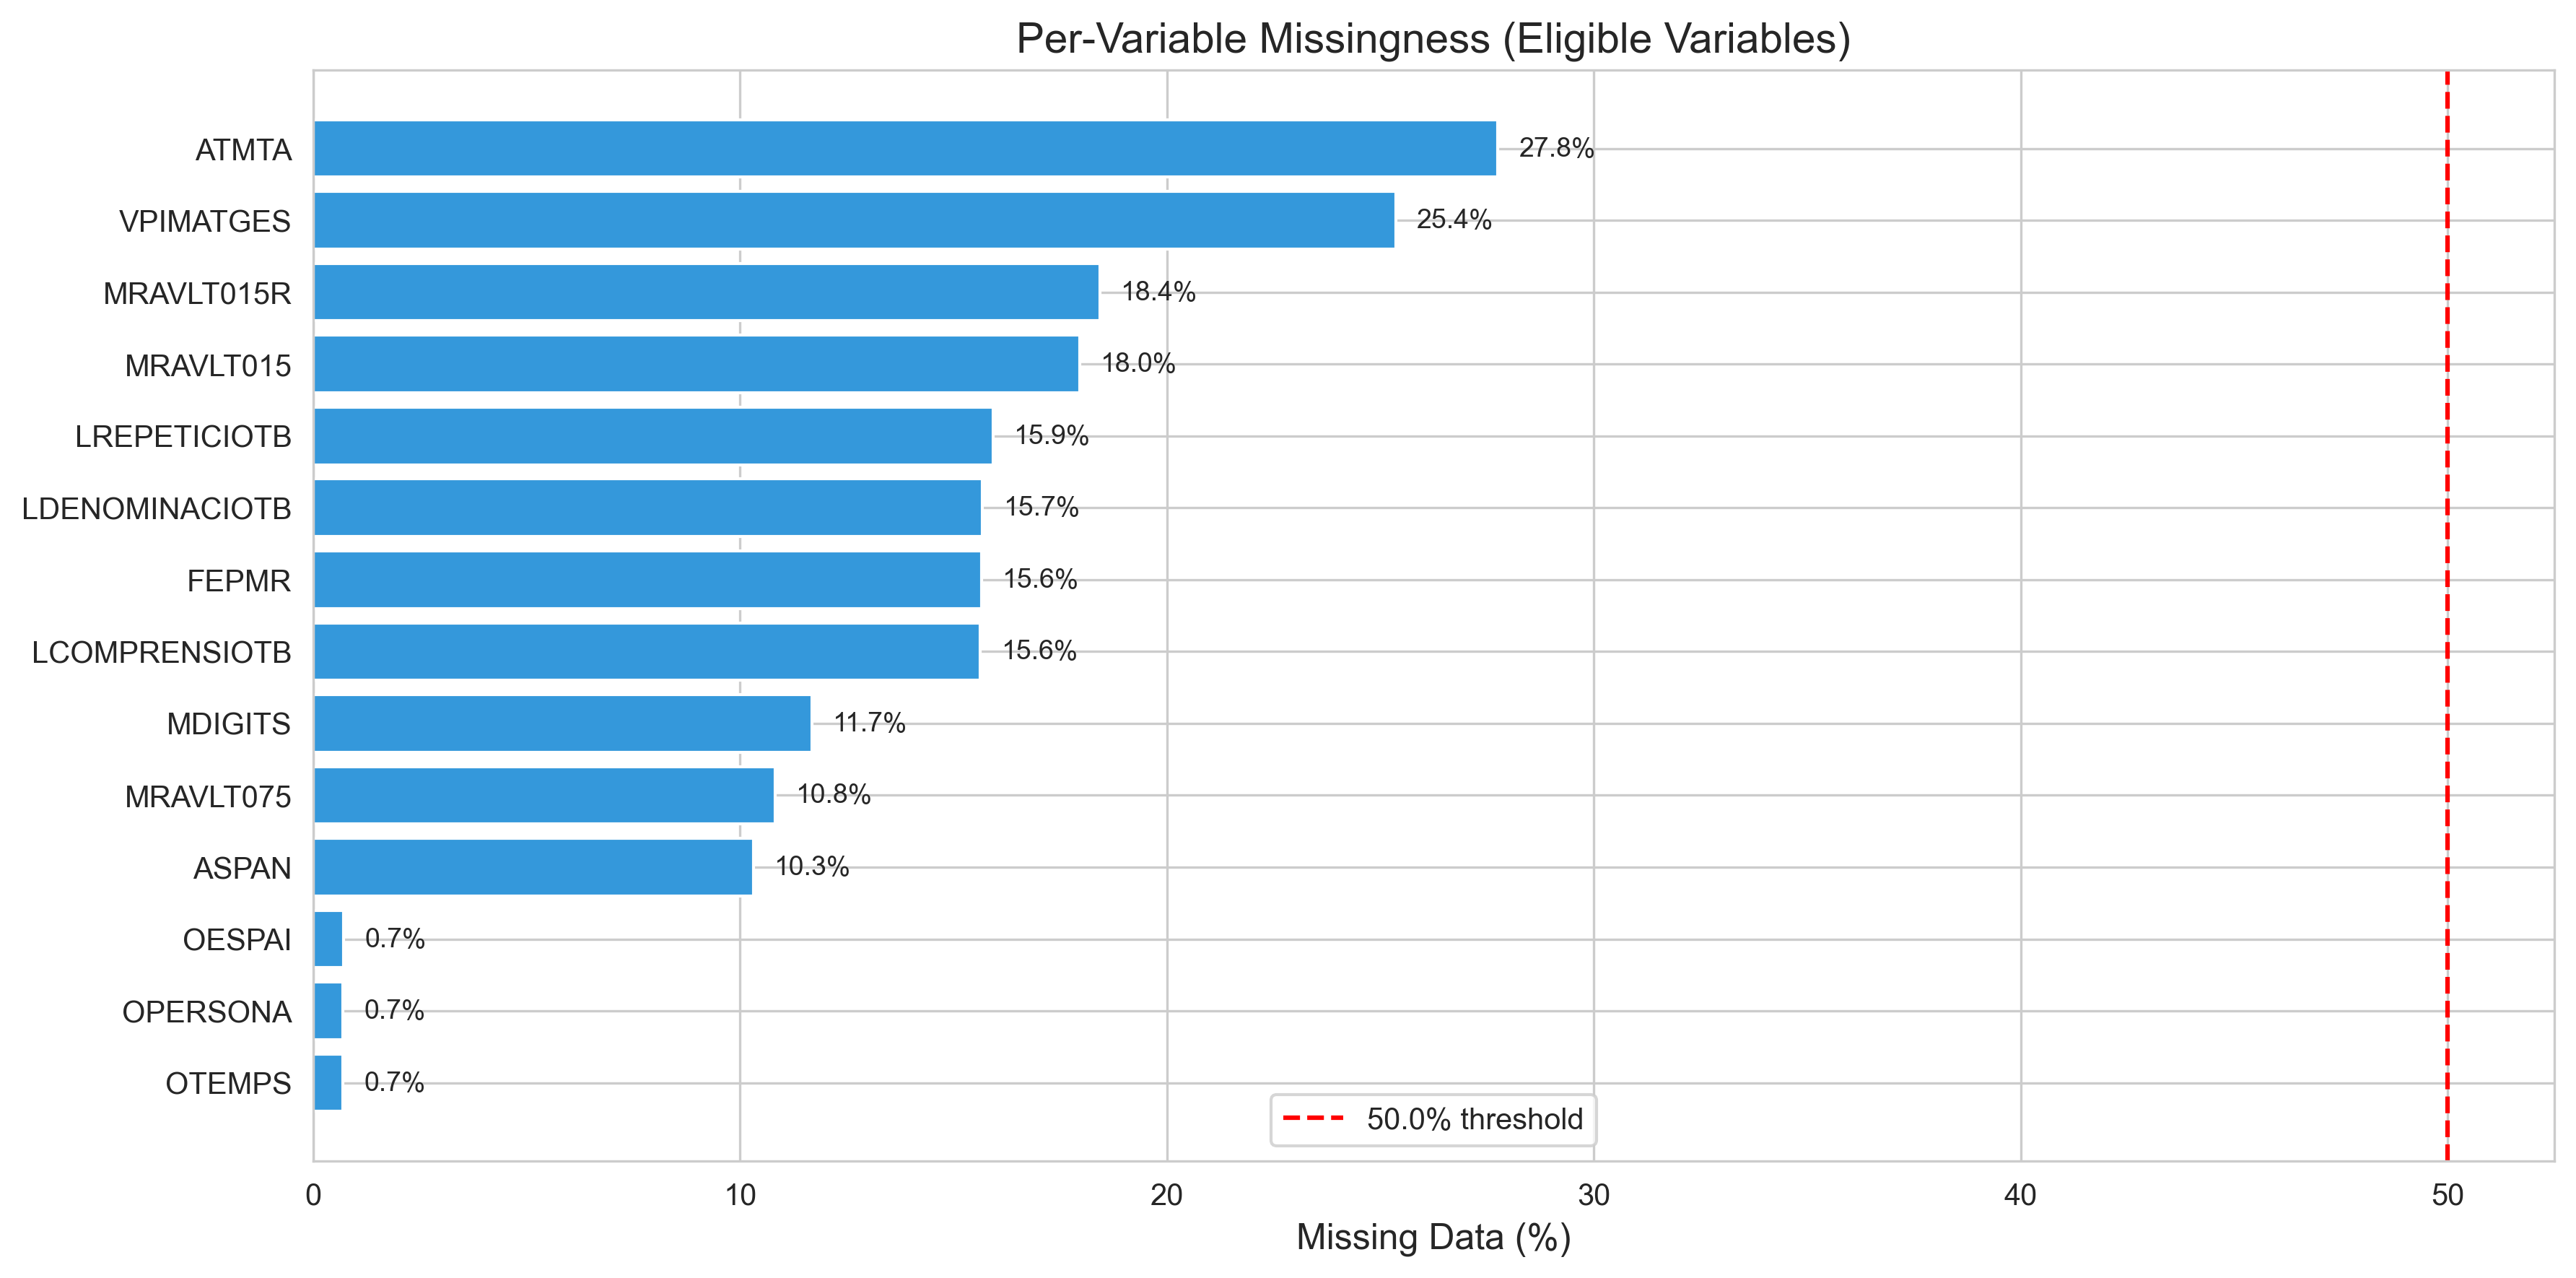
\includegraphics[width=0.9\textwidth]{Figures/missingness_barplot.png}
\caption[Missingness rates by variable]{Proportion of missing values for each cognitive variable, ordered by missingness rate. Specialised assessments show higher missingness than the routinely administered screening measures.}
\label{fig:missingness_barplot}
\end{figure}

A co-occurrence heatmap (not shown) reveals blocks of variables that are absent together, a pattern consistent with a missing-at-random mechanism \parencite{rubin1976inference, little2019statistical}. Such dependency favours conditional imputation over naive substitution. Among observed values, within-domain correlations are strong and cross-domain associations are more modest, probably reflecting shared variance with general cognitive ability \parencite{lezak2012neuropsychological}. The clustering results later make this shared severity dimension explicit.

%----------------------------------------------------------------------------------------
%	SECTION 2
%----------------------------------------------------------------------------------------

\section{Imputation Results}

To prepare the datasets for downstream clustering, I evaluated all ten imputation methods, shown in Figures~\ref{fig:imputation_comparison} and \ref{fig:imputation_comparison_b}. Mean Imputation behaves differently from the other methods because, as expected for single-value imputation, it compresses variance \parencite{rubin1987multiple}. The remaining nine methods preserve the marginal distributions more closely. Donor-based methods such as KNN and PMM retain more discrete structure, while model-based approaches such as MICE, MissForest, and EM produce smoother continuous reconstructions.

\begin{figure}[htbp]
\centering
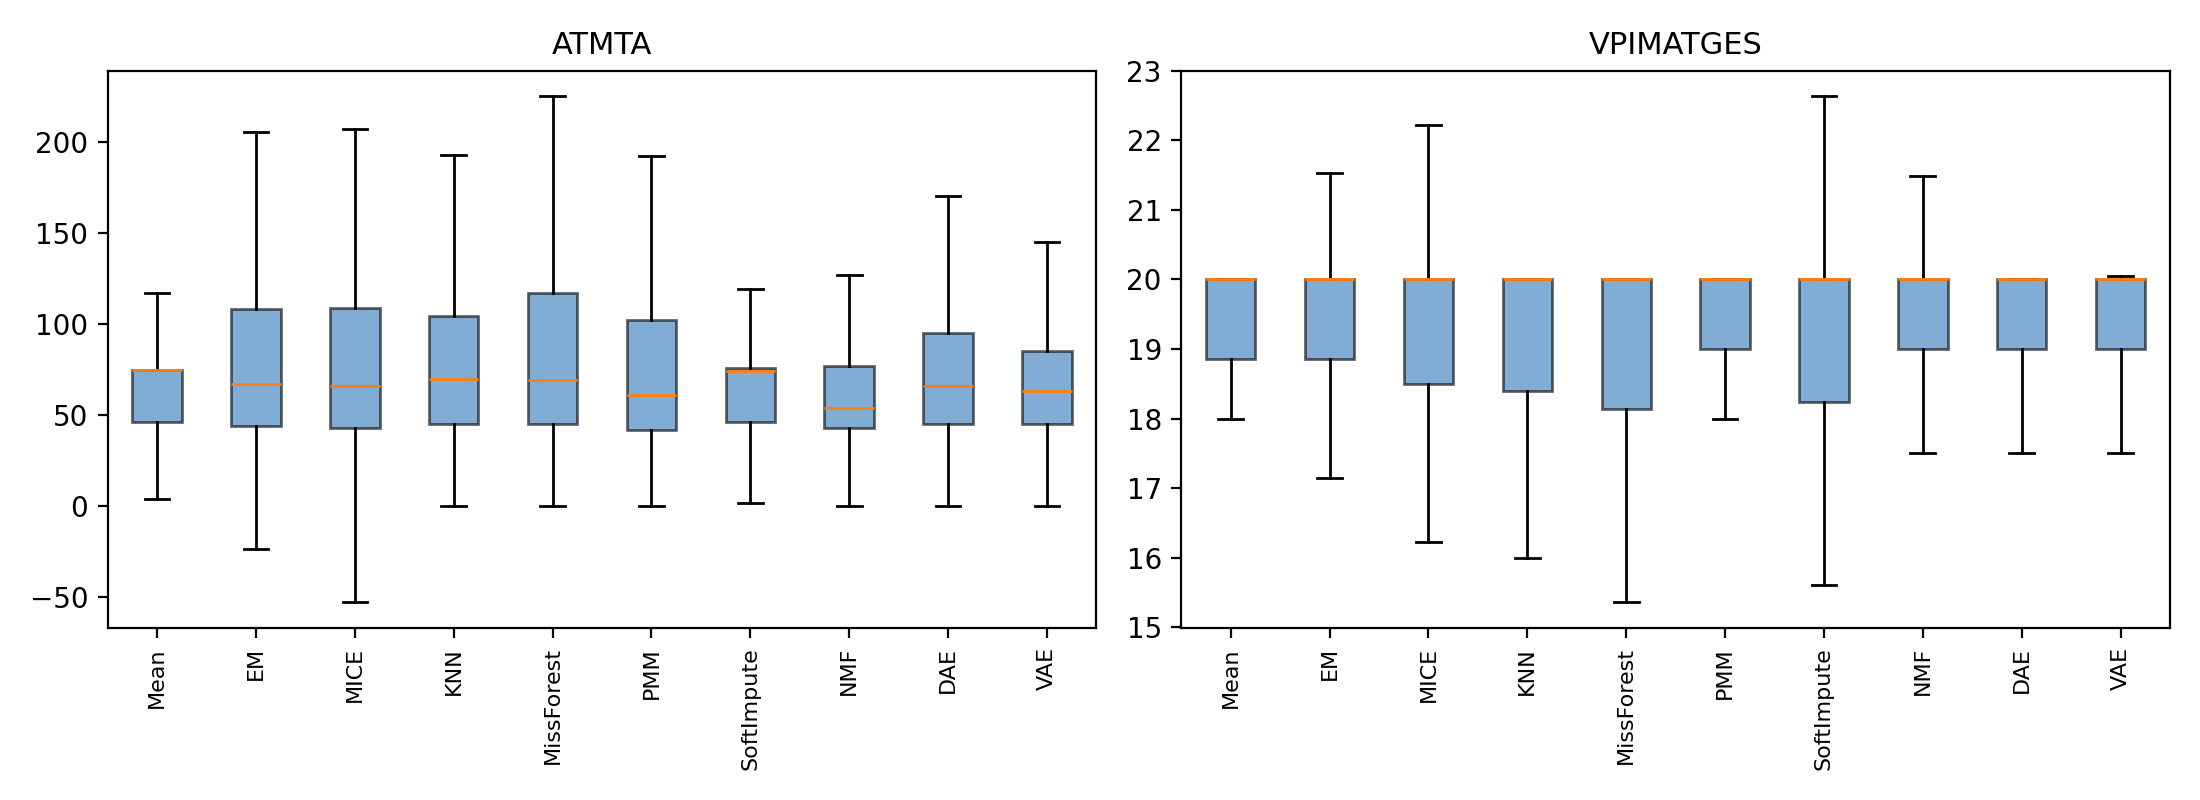
\includegraphics[width=0.95\textwidth]{Figures/imputation_comparison_boxplots_a.png}
\caption[Imputation comparison (ATMTA, VPIMATGES)]{Distribution comparison across ten imputation methods for ATMTA and VPIMATGES. Mean Imputation compresses variance; model-based methods preserve distributional shape.}
\label{fig:imputation_comparison}
\end{figure}

\begin{figure}[htbp]
\centering
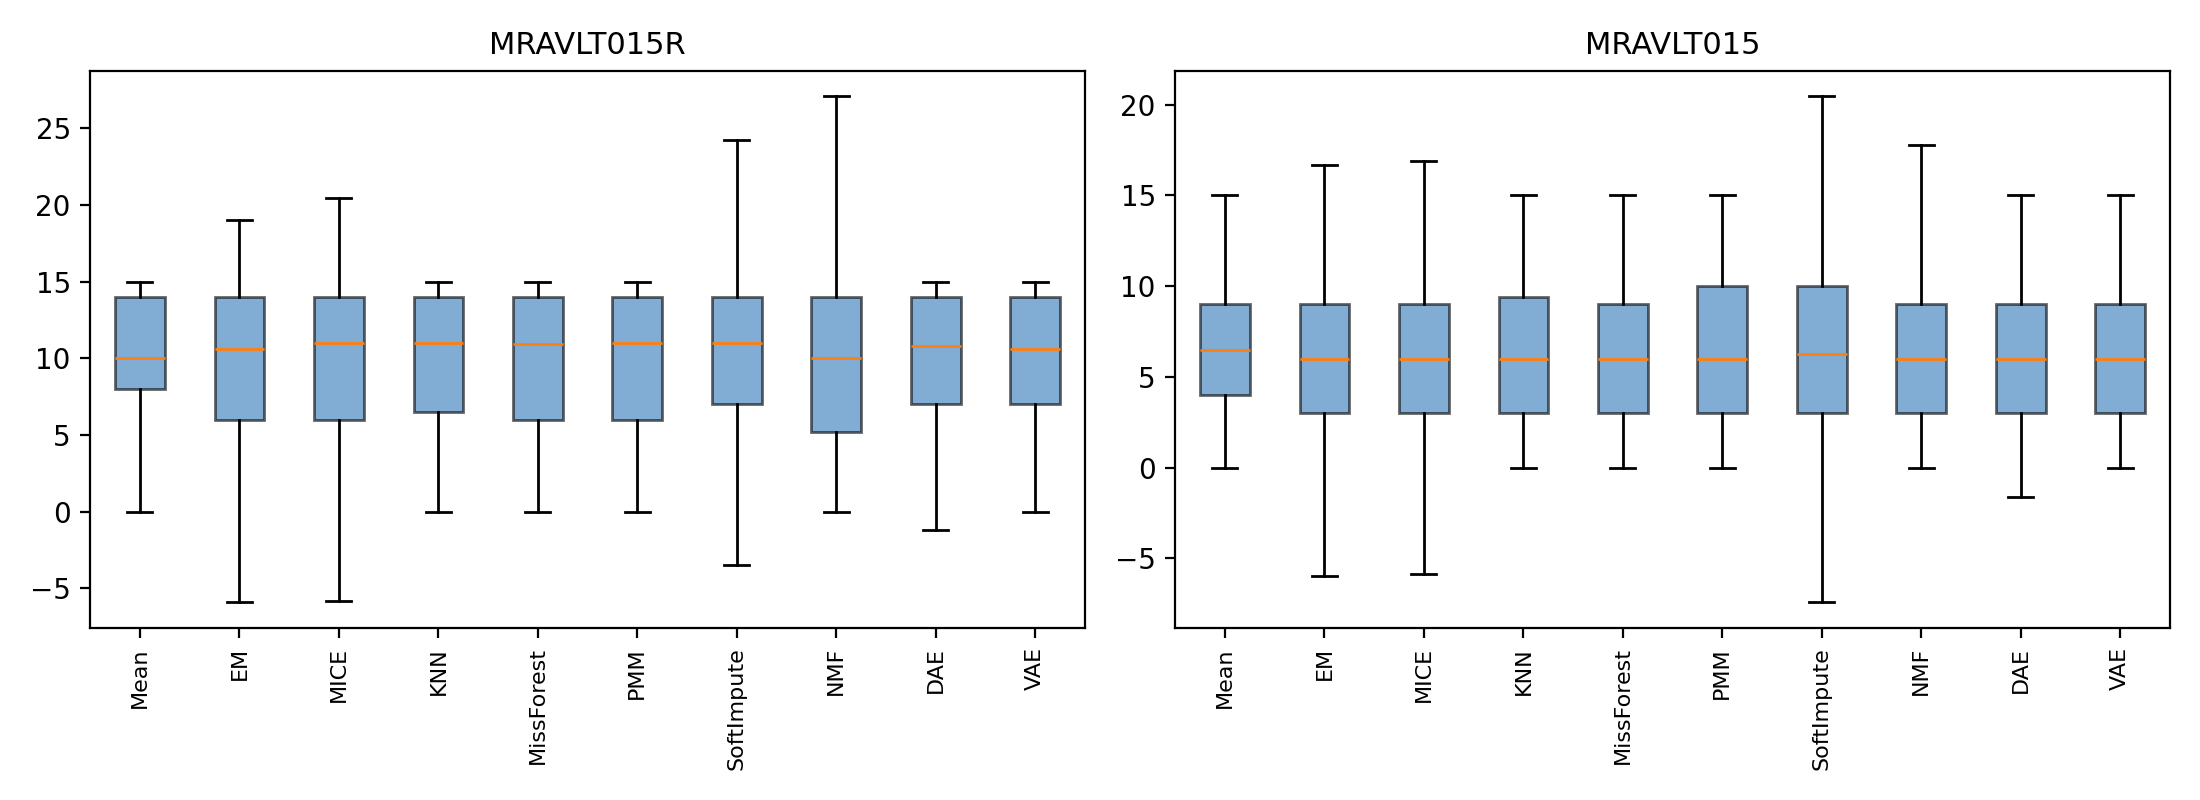
\includegraphics[width=0.95\textwidth]{Figures/imputation_comparison_boxplots_b.png}
\caption[Imputation comparison (MRAVLT015R, MRAVLT015)]{Distribution comparison for MRAVLT015R and MRAVLT015. Deep learning methods (DAE, VAE) closely match model-based methods.}
\label{fig:imputation_comparison_b}
\end{figure}

%----------------------------------------------------------------------------------------
%	SECTION 3
%----------------------------------------------------------------------------------------

\section{Baseline and Primary Clustering}

K-Means and Gaussian mixture models were fitted for $k = 2,\dots,6$ as baselines before the primary pipeline was applied. Neither method identified a clear optimum. The K-Means elbow plot declined steadily without a sharp inflection, and silhouette scores peaked at $k = 2$ before decreasing. GMM produced a similar absence of a stable minimum. These baselines suggest that the cognitive profile space behaves more like a continuum than a set of separated islands, motivating the use of density-based clustering \parencite{scikit2011learn}.

\begin{sloppypar}
For the UMAP+HDBSCAN combination, the hyperparameters I settled on were: \texttt{n\_components}$= 8$, \texttt{n\_neighbors}$= 15$, and \texttt{min\_dist}$= 0.0$ for UMAP (to allow for tight packing in the embedding space \parencite{mcinnes2018umap}); and for HDBSCAN, \texttt{min\_cluster\_size}$= 1000$ and \texttt{min\_samples}$= 50$ with \texttt{cluster\_selection\_method}$= \text{eom}$ and \texttt{epsilon}$= 0.0$. I chose a large cluster size to ensure that only substantive groupings are retained.
\end{sloppypar}

In the MICE-imputed data, HDBSCAN identified three clusters. The high-density core, containing approximately 92\% of assessments, achieved a silhouette score of 0.598 (Table~\ref{tab:method_summary}). Boundary observations were then assigned to substantive clusters by the $k$-nearest-neighbour reassignment step, producing labels for all 17{,}406 assessments, 0\% residual noise, and an overall silhouette of 0.526. The reduction in silhouette is expected because reassigned boundary cases are intrinsically less separable, but the final value remains substantially above the baseline. Figure~\ref{fig:tsne_umap} compares t-SNE and UMAP projections with HDBSCAN assignments colour-coded; UMAP delineates the boundaries more clearly, consistent with its stronger preservation of local and global structure \parencite{mcinnes2018umap, vandermaaten2008tsne}.

\begin{figure}[htbp]
\centering
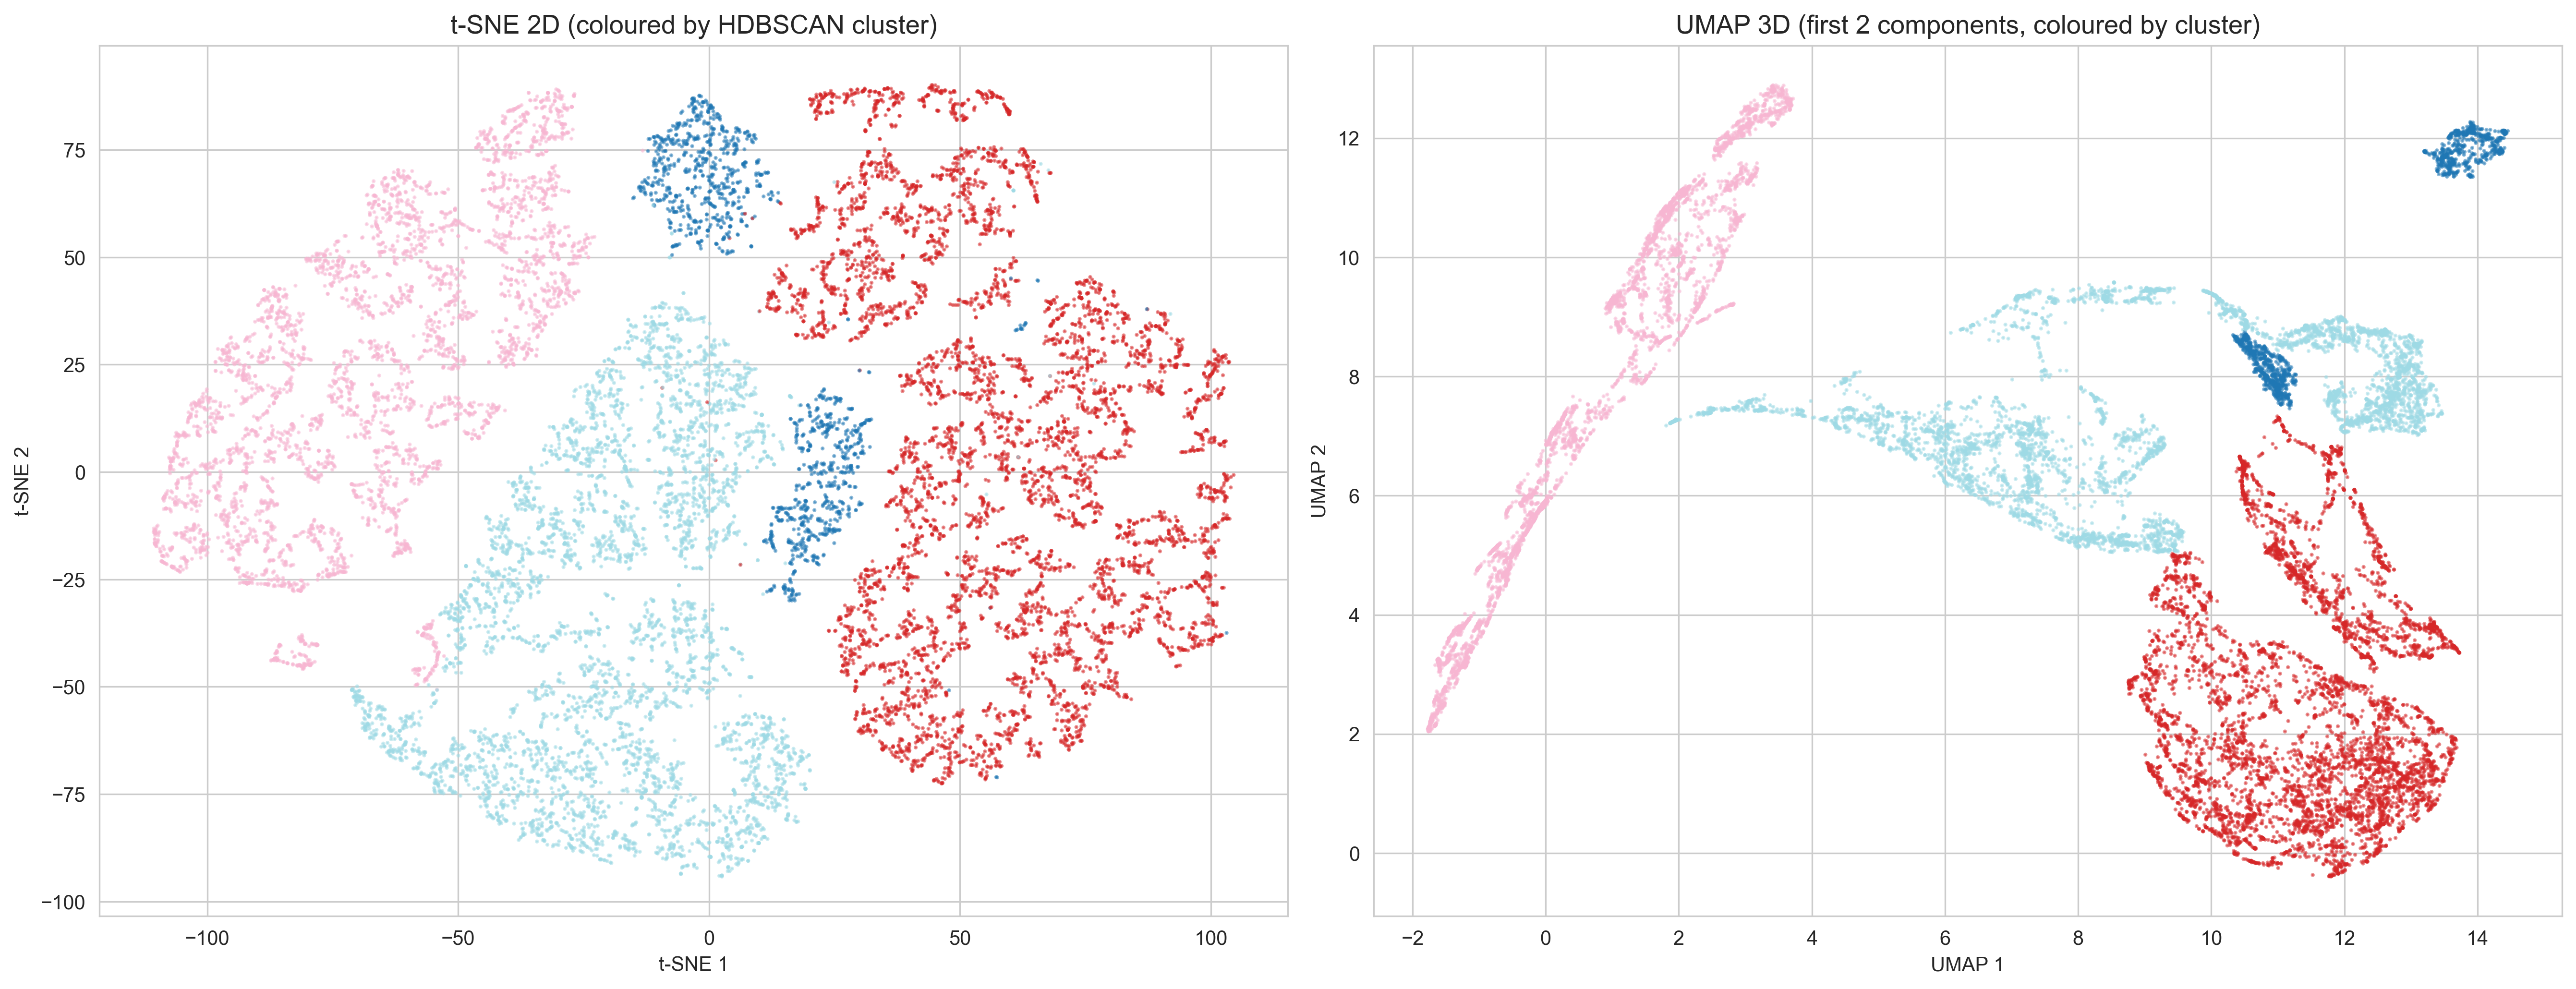
\includegraphics[width=0.9\textwidth]{Figures/tsne_umap_clusters.png}
\caption[t-SNE and UMAP cluster projections]{Two-dimensional projections using t-SNE (left) and UMAP (right) with HDBSCAN cluster assignments colour-coded. UMAP reveals more clearly separated cluster regions.}
\label{fig:tsne_umap}
\end{figure}

The final solution contains three groups ordered by cognitive level: \emph{Above-Average} ($n = 6{,}725$), \emph{Near-Normal} ($n = 6{,}328$), and \emph{Global Impairment} ($n = 4{,}353$). All assessments are assigned. The important distinction is not profile shape, but position along a severity axis.

%----------------------------------------------------------------------------------------
%	SECTION 4
%----------------------------------------------------------------------------------------

\section{Cognitive Profiles of the Clusters}\label{sec:cluster_profiles}

I computed domain-level profiles to describe the clusters. Figure~\ref{fig:radar_profiles} shows the mean domain $z$-score for the three tiers (left) and the domain contributions from a surrogate classifier (right).

\begin{figure}[!ht]
\centering
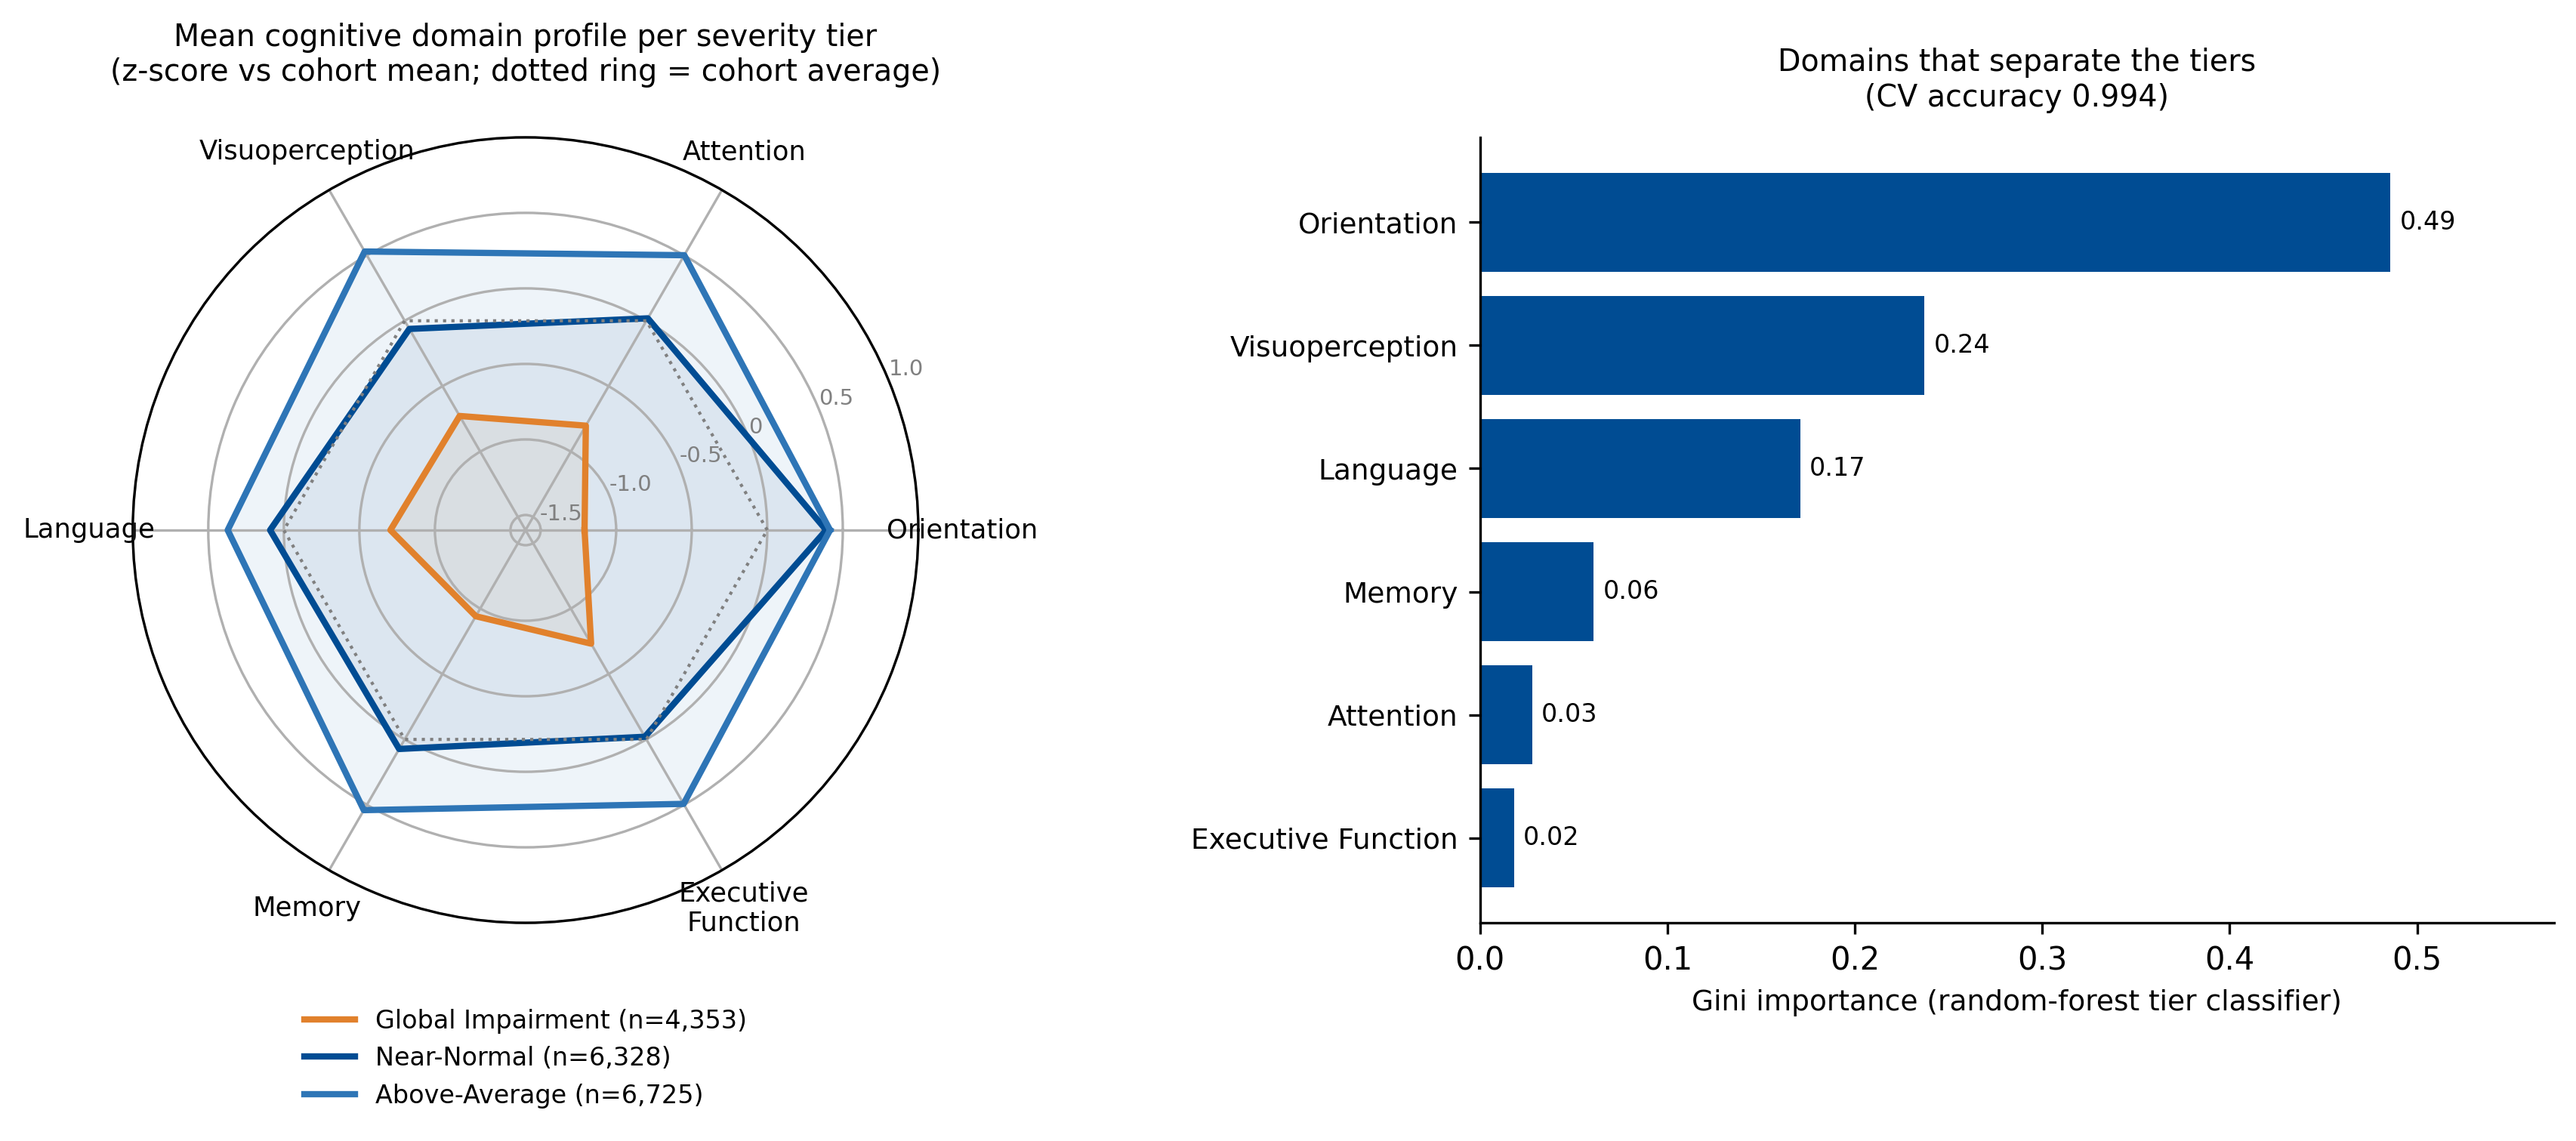
\includegraphics[width=\textwidth]{Figures/cognitive_radar_profiles.png}
\caption[Cognitive domain severity profiles]{Left: mean cognitive domain score per tier, expressed as a $z$-score from the cohort mean (dotted ring = cohort average). The three polygons are roughly concentric (every domain moves together), so the tiers differ in overall level rather than in profile \emph{shape}. Right: Gini importance from a random-forest surrogate that recovers the tier labels from the domain scores (accuracy 0.994). As the labels derive from those same scores, this panel re-describes the partition's decision boundaries rather than measuring independent importance, and the ordering is sensitive to inter-domain correlation (§\ref{sec:feature_importance}); it should not be read as evidence that attention is clinically unimportant.}
\label{fig:radar_profiles}
\end{figure}

The defining feature of the solution is the near-concentric geometry of the three profiles. The \emph{Above-Average} tier lies above the cohort mean in all six domains ($z$ from $+0.37$ to $+0.54$); the \emph{Global Impairment} tier lies below it in all six ($z$ from $-0.71$ to $-1.21$); and the \emph{Near-Normal} tier remains close to the cohort average. These are not profiles in which one domain is selectively impaired and another spared. They are ordered bands along an \emph{overall-severity} gradient. Principal-component analysis supports that reading: the first component has near-equal positive loadings on every domain and explains 56\% of the variance, while no subsequent component exceeds 13\%. The recovered structure is therefore primarily one-dimensional.

%----------------------------------------------------------------------------------------
%	SECTION 5
%----------------------------------------------------------------------------------------

\section{Hypothesis 1: Discrete, Stable Clusters}\label{sec:h1_results}

Hypothesis~1 predicted discrete and stable cognitive clusters. The pre-registered criterion required at least 8 of the 10 imputation methods to satisfy both thresholds: mean silhouette above 0.40 and pre-KNN noise below 0.30. Two analyses were used to evaluate this criterion.

\textbf{Per-method bootstrap.} For each method, HDBSCAN was re-fitted on 50 bootstrap resamples of the UMAP embedding. All ten methods exceeded the 8/10 target. Median core silhouettes fell in the 0.50--0.60 range, close to the single-run values in Table~\ref{tab:method_summary}, and pre-KNN noise ranged from 0.03 to 0.17. Cluster count varied between three and five, with four as the mode and three in the MICE reference solution. That variation is consistent with discretising a continuous severity gradient: the number of density-defined bands depends partly on resolution, not solely on a fixed latent class count.

\textbf{Per-cluster core Jaccard.} I then examined how reproducibly individual clusters were recovered using Hennig (2007) matching on the pre-KNN HDBSCAN labels. For the MICE tiers, the core Jaccards were 0.63 for \emph{Above-Average}, 0.62 for \emph{Global Impairment}, and 0.47 for \emph{Near-Normal}. The two outer tiers are close to the conventional 0.7 stability threshold. The \emph{Near-Normal} tier is less stable, as expected for the middle band of a gradient, where boundary patients can switch between adjacent tiers across resamples.

The data support Hypothesis~1. All ten imputation methods meet the pre-registered silhouette and noise thresholds, and Hennig matching recovers the two extreme MICE tiers with per-cluster core Jaccards above 0.6. The result is a stable severity stratification, not strong evidence for qualitatively distinct phenotypes.

%----------------------------------------------------------------------------------------
%	SECTION 6
%----------------------------------------------------------------------------------------

\section{Hypothesis 2: Imputation Sensitivity}\label{sec:h2_results}

\begin{sloppypar}
To test Hypothesis~2---which predicted that the patient clusters would remain robust regardless of the imputation method---I implemented a standardised analytical pipeline. This shared design ensured that the effects of the imputation were completely isolated. The workflow proceeded as follows: the \texttt{StandardScaler}, UMAP, and $k$-means models were fitted once on the MICE-imputed data and then applied (via \texttt{transform}/\texttt{predict}) to every other method, so that the imputed values were the only thing varying. I quantified agreement with the Adjusted Rand Index (ARI; \parencite{hubert1985comparing}) and Normalised Mutual Information (NMI; \parencite{vinh2010information}).
\end{sloppypar}

Figure~\ref{fig:h2_ari_nmi} indicates substantial membership overlap across imputation methods. Since an ARI of 1 denotes perfect agreement and 0 denotes chance-level agreement, the 0.50 threshold for H2 represents a demanding criterion for concordance. The mean ARI across the $\binom{10}{2} = 45$ method pairs was 0.710 (median 0.739), and no pair fell below 0.50 (range 0.509--0.880). Excluding Mean Imputation barely changed the mean, which fell to 0.708. Several method pairs produced near-identical partitions, including EM--DAE (ARI 0.880), DAE--VAE (0.863), and EM--VAE (0.828).

\begin{figure}[!ht]
\centering
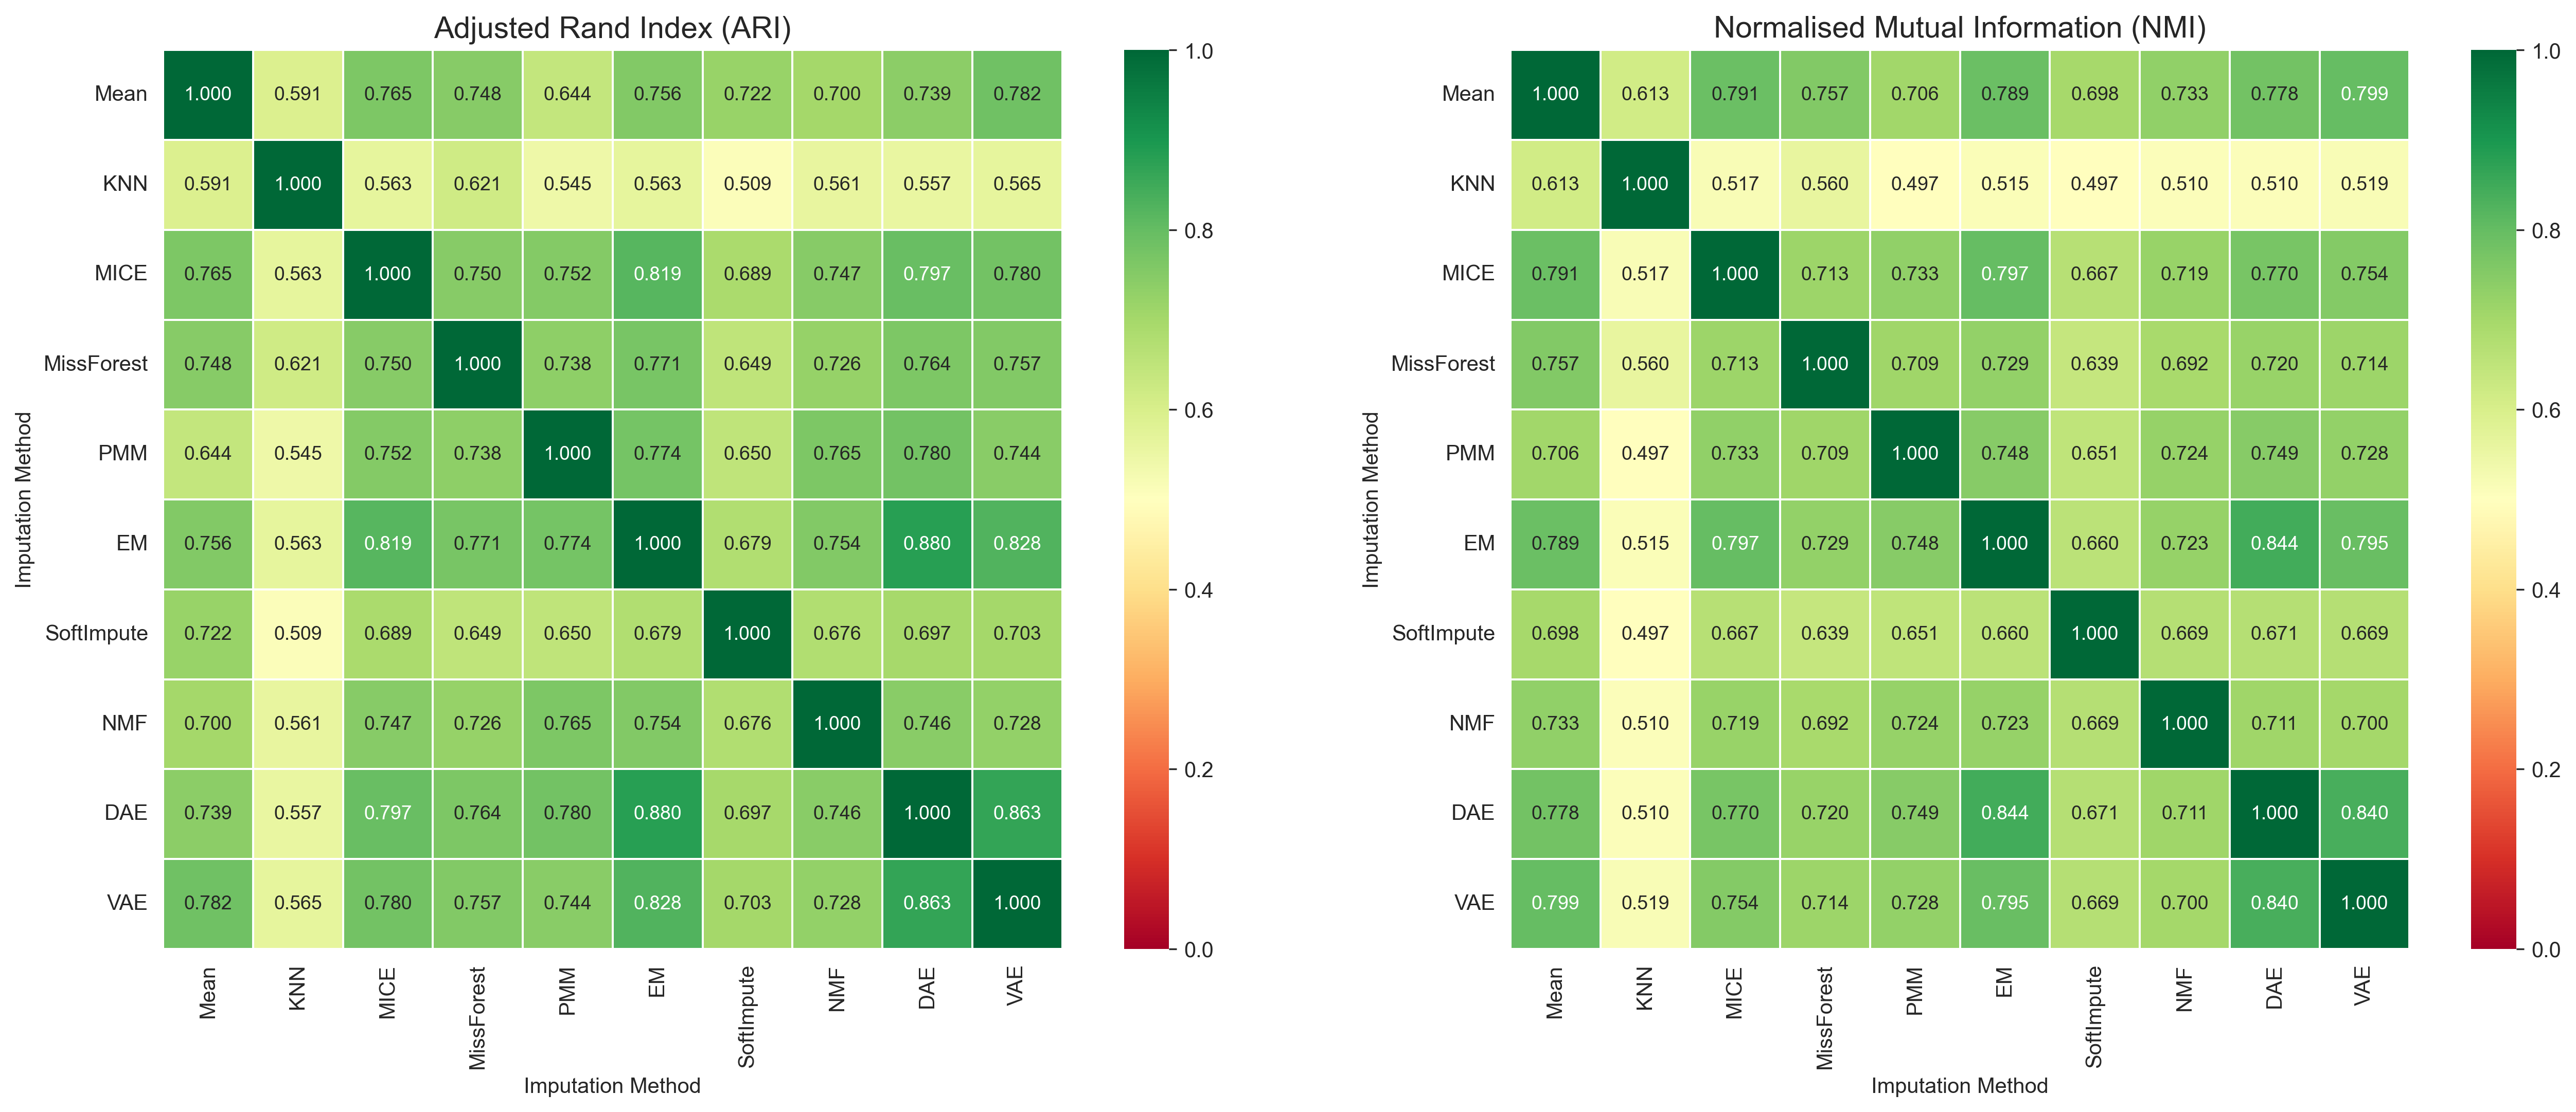
\includegraphics[width=0.65\textwidth]{Figures/h2_ari_nmi_heatmap.png}
\caption[ARI and NMI heatmap across imputation methods]{Pairwise Adjusted Rand Index (top) and Normalised Mutual Information (bottom) across the ten imputation methods. Agreement is high throughout; KNN shows the lowest agreement with the smoother model-based methods.}
\label{fig:h2_ari_nmi}
\end{figure}

At assessment level, instability was moderately associated with the fraction of imputed values ($r = 0.474$, $p < 0.001$). More missingness meant less stable tier assignment. The imputation effect is therefore concentrated in assessments where the observed evidence is sparse.

To derive a consensus label, per-method labels were aligned with the Hungarian algorithm, maximising one-to-one overlap between label sets. A majority vote was then taken across all ten methods for each assessment, and confidence was defined as the proportion of methods agreeing with that vote. Mean confidence was 0.929; 86.2\% of the cohort received a high-confidence tier label ($\ge 0.8$). Discordant cases were concentrated near boundaries between severity tiers and should be flagged rather than interpreted as equally certain assignments.

\begin{figure}[!ht]
\centering
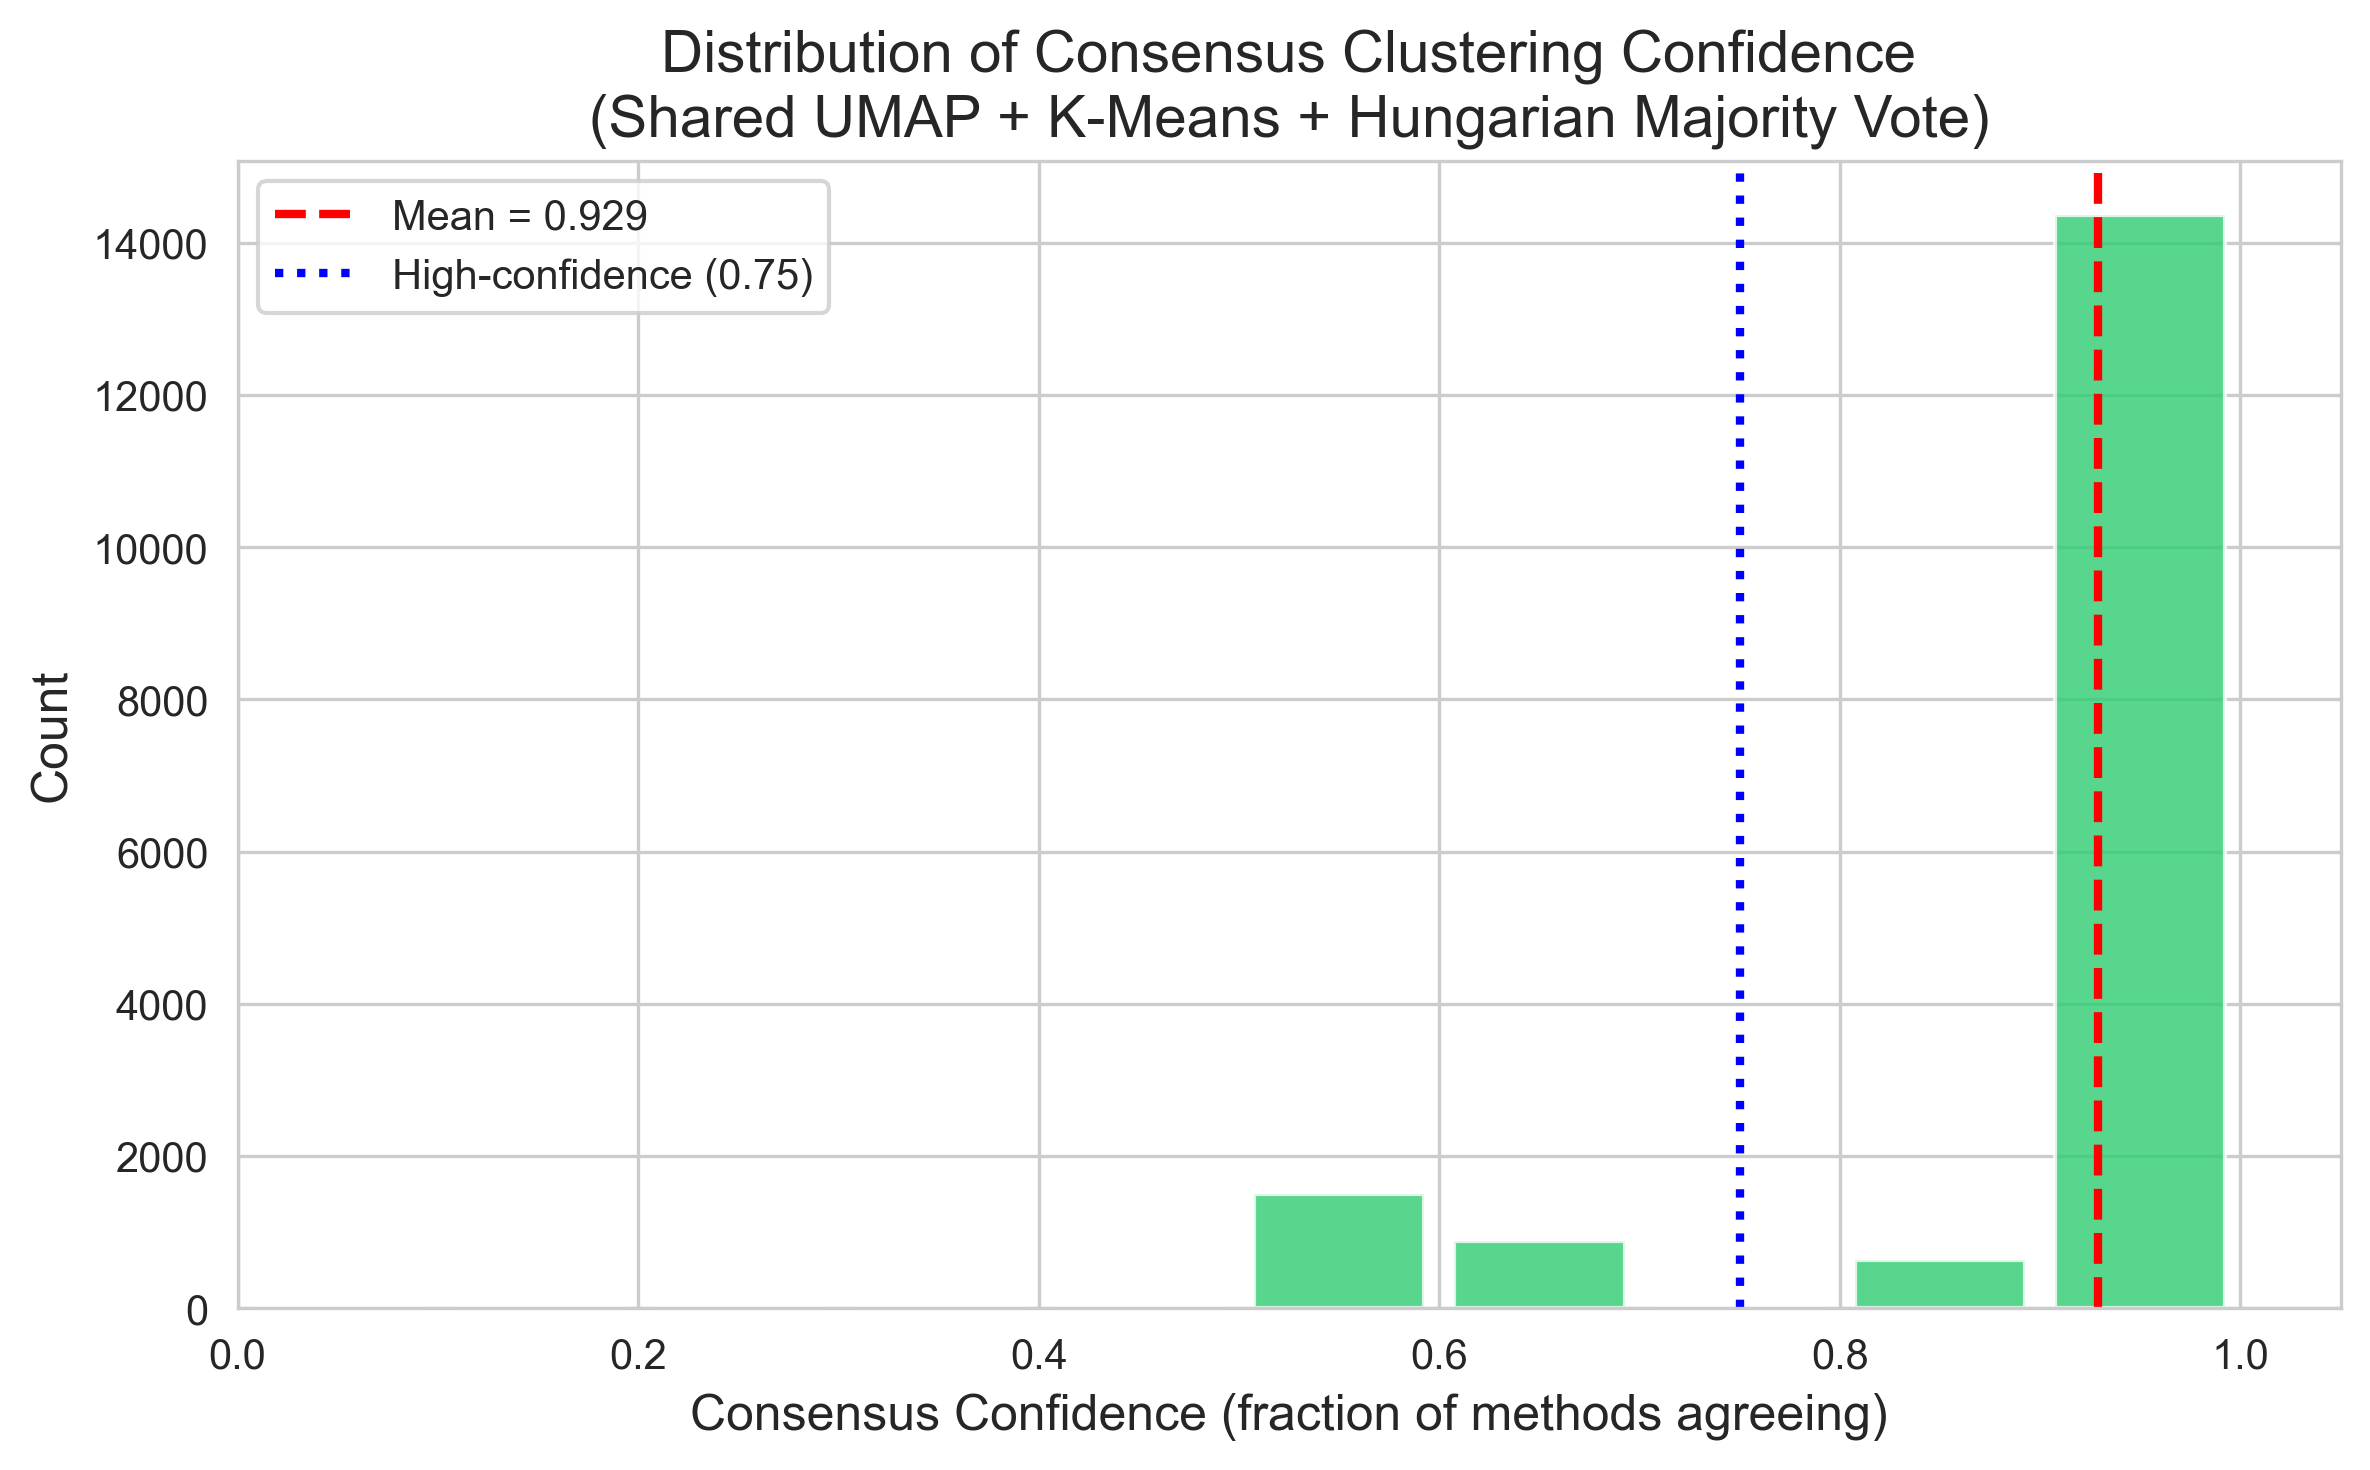
\includegraphics[width=0.85\textwidth]{Figures/h2_consensus_confidence.png}
\caption[Consensus clustering confidence]{Distribution of consensus confidence scores (proportion of methods agreeing on assignment). Higher values indicate assessments whose assignment is robust across imputation methods.}
\label{fig:h2_consensus}
\end{figure}

Hypothesis~2 is supported. The mean ARI of 0.710 (95\% bootstrap CI [0.704, 0.716]) and high consensus confidence (mean 0.929) show that severity tiers are recovered reliably across imputation methods. After Holm--Bonferroni correction across the 45 tests, 44 reject $H_0$:~ARI~$\le 0.5$ at $\alpha = 0.05$ (Section~\ref{sec:robustness}). KNN--SoftImpute is the sole exception, with a bootstrap mean ARI of 0.509, close to the threshold.

\begin{figure}[!ht]
\centering
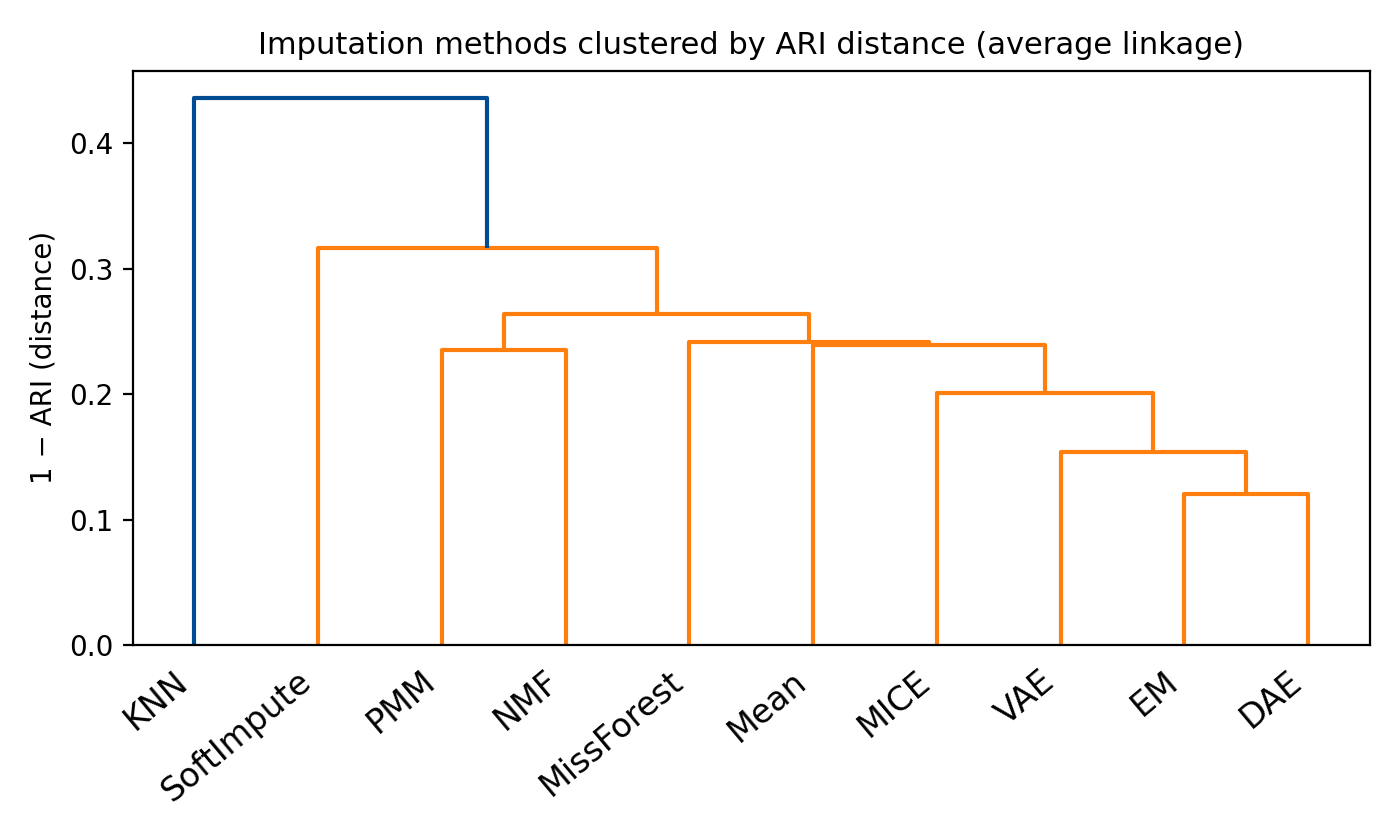
\includegraphics[width=0.85\textwidth]{Figures/h2_method_dendrogram.png}
\caption[Method dendrogram based on ARI distance]{Dendrogram of imputation methods using average-linkage clustering on ARI-based distances. KNN forms the most distinct branch, while the smoother model-based methods group tightly together.}
\label{fig:h2_dendrogram}
\end{figure}

\clearpage

%----------------------------------------------------------------------------------------
%	SECTION 7
%----------------------------------------------------------------------------------------

\section{Hypothesis 3: Clinical Unit Association}\label{sec:h3_results}

Under Hypothesis~3 I anticipated a significant association between cluster membership and clinical-unit assignment. To test this I ran a chi-squared test of independence and calculated Cram\'{e}r's V as a measure of effect size \parencite{cramer1946mathematical}.

The association was strong statistically: $\chi^2 = 911.3$ ($p \approx 4 \times 10^{-156}$), with Cram\'{e}r's V = 0.162. By Cohen's conventions, the effect is small; by the pre-registered threshold, it is meaningful. Cognitive severity tier therefore contributes information about patient placement beyond diagnostic category alone. Figure~\ref{fig:h3_heatmap} shows the concentration of specific tiers within particular units.

\begin{figure}[htbp]
\centering
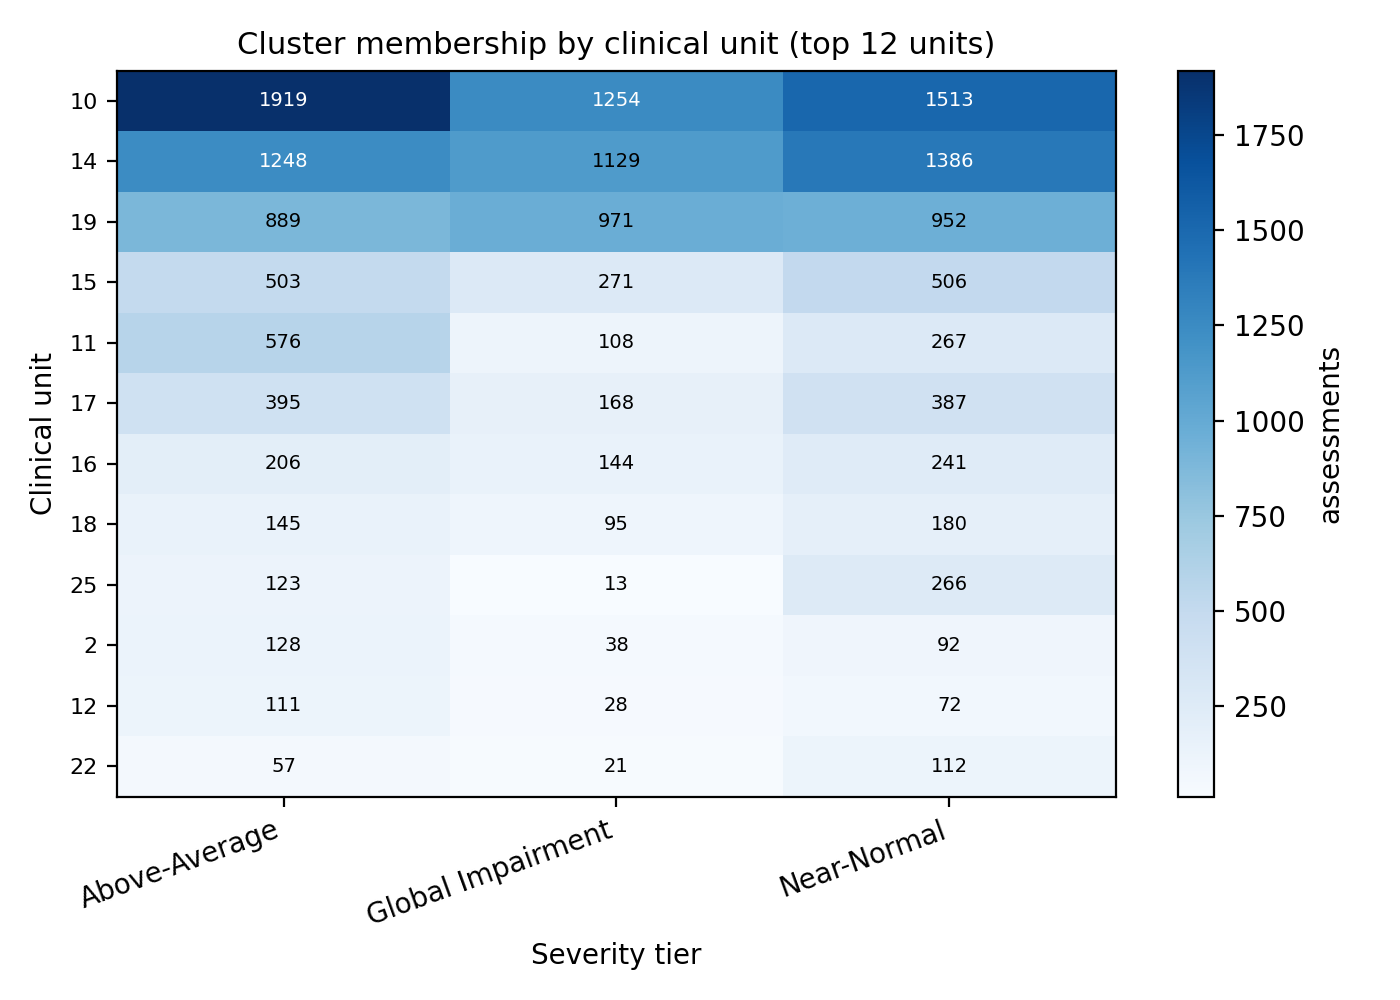
\includegraphics[width=0.9\textwidth]{Figures/h3_clinical_unit_heatmap.png}
\caption[Clinical unit by cluster heatmap]{Heatmap of cluster membership (columns) by clinical unit (rows). Cell colours indicate observed frequency. Certain severity tiers are concentrated within specific units.}
\label{fig:h3_heatmap}
\end{figure}

The Cochran-Mantel-Haenszel test, stratified by diagnosis group, was then used to assess confounding by diagnostic category. The CMH result indicated that the association persisted after controlling for diagnosis \parencite{cochran1954some}. Rubin-pooled multiple imputation (Section~\ref{sec:robustness}) produced a pooled Cram\'{e}r's V of 0.154 [0.049, 0.259], consistent with the single-draw estimate and above the hypothesis threshold. Hypothesis~3 is supported.

%----------------------------------------------------------------------------------------
%	SECTION 8
%----------------------------------------------------------------------------------------

\section{Hypothesis 4: Feature Engineering}\label{sec:h4_results}

The central prediction was that aggregating features at the domain level would yield more robust clustering than operating on individual variables. I evaluated both representations across three metrics: silhouette scores, the condition number, and the Variance Inflation Factor (VIF).

Domain-level aggregation produced a slightly higher mean silhouette score than the variable-level representation (0.481 vs.\ 0.473; Figure~\ref{fig:h4_comparison}). The more important change occurred in feature-space conditioning. Mean VIF fell from 2.77 to 1.88, and the condition number fell from 61.7 to 11.8. Because high VIF values indicate multicollinearity, and high condition numbers can distort distance computations used by UMAP and HDBSCAN, this reduction is methodologically consequential. Aggregation reduces redundancy while preserving the latent cognitive constructs represented by the tests \parencite{lezak2012neuropsychological}.

\begin{figure}[htbp]
\centering
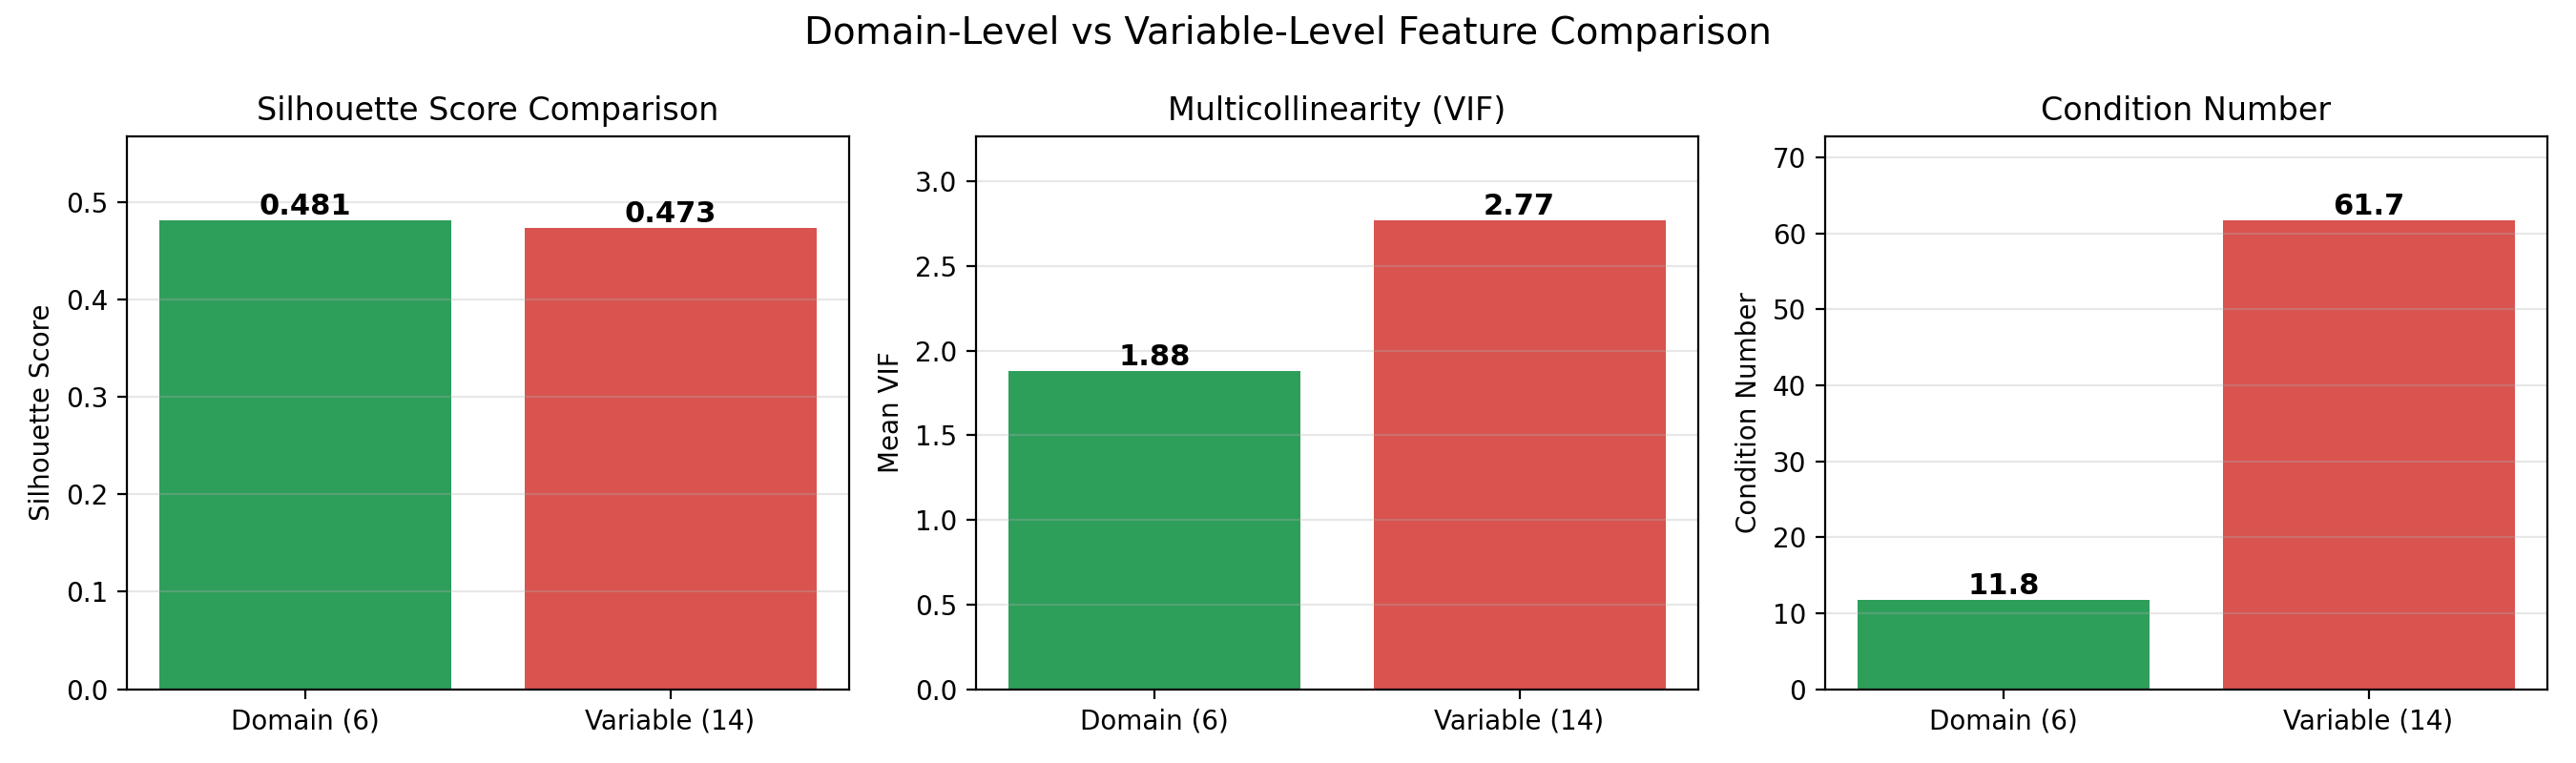
\includegraphics[width=0.95\textwidth]{Figures/h4_domain_vs_variable.png}
\caption[Domain vs variable: silhouette, VIF, conditioning]{Domain-aggregated versus variable-level features on silhouette (0.481 vs 0.473), mean VIF (1.88 vs 2.77), and condition number (11.8 vs 61.7). Domain aggregation produces comparably separated but far less collinear, better-conditioned features.}
\label{fig:h4_comparison}
\end{figure}

Hypothesis~4 is therefore supported. Domain-level feature engineering improves numerical stability without sacrificing cluster separation.

%----------------------------------------------------------------------------------------
%	SECTION 9
%----------------------------------------------------------------------------------------

\section{Feature Importance Analysis}\label{sec:feature_importance}

For this analysis, I trained a Random Forest surrogate on the MICE-imputed domain scores, using the tier labels as the target. It achieved 99.4\% accuracy in 5-fold cross-validation. This result describes the separability of the tiers in domain space; it does not independently validate the clustering. Because the tier labels were generated from the same domain scores through UMAP+HDBSCAN, a classifier that recovers them is effectively reconstructing the clustering boundaries. The near-perfect accuracy therefore shows that the ordered severity tiers are highly separable in domain space.

As an interpretability aid, the Gini and permutation rankings placed orientation first (Gini 0.49), followed by visuoperception (0.24) and language (0.17), with attention (0.03) and executive function (0.02) lower in the ranking (Figure~\ref{fig:feature_importance}). This ordering should be interpreted cautiously. It is internal to the clustering procedure and is partly circular. In addition, Gini importance is biased when predictors are correlated \parencite{boulesteix2012overview}. The six domains are strongly positively correlated, consistent with the cognitive positive manifold and with the first principal component described in §\ref{sec:cluster_profiles}. Once a tree has split on a highly correlated domain such as orientation, attention can appear redundant. Its low importance score should therefore not be interpreted as evidence that attention is clinically unimportant. The concentric profiles and principal-component loadings in Figure~\ref{fig:radar_profiles}, rather than the surrogate importance ranking, determine whether the tiers represent overall severity or a domain-specific dissociation.

\begin{figure}[htbp]
\centering
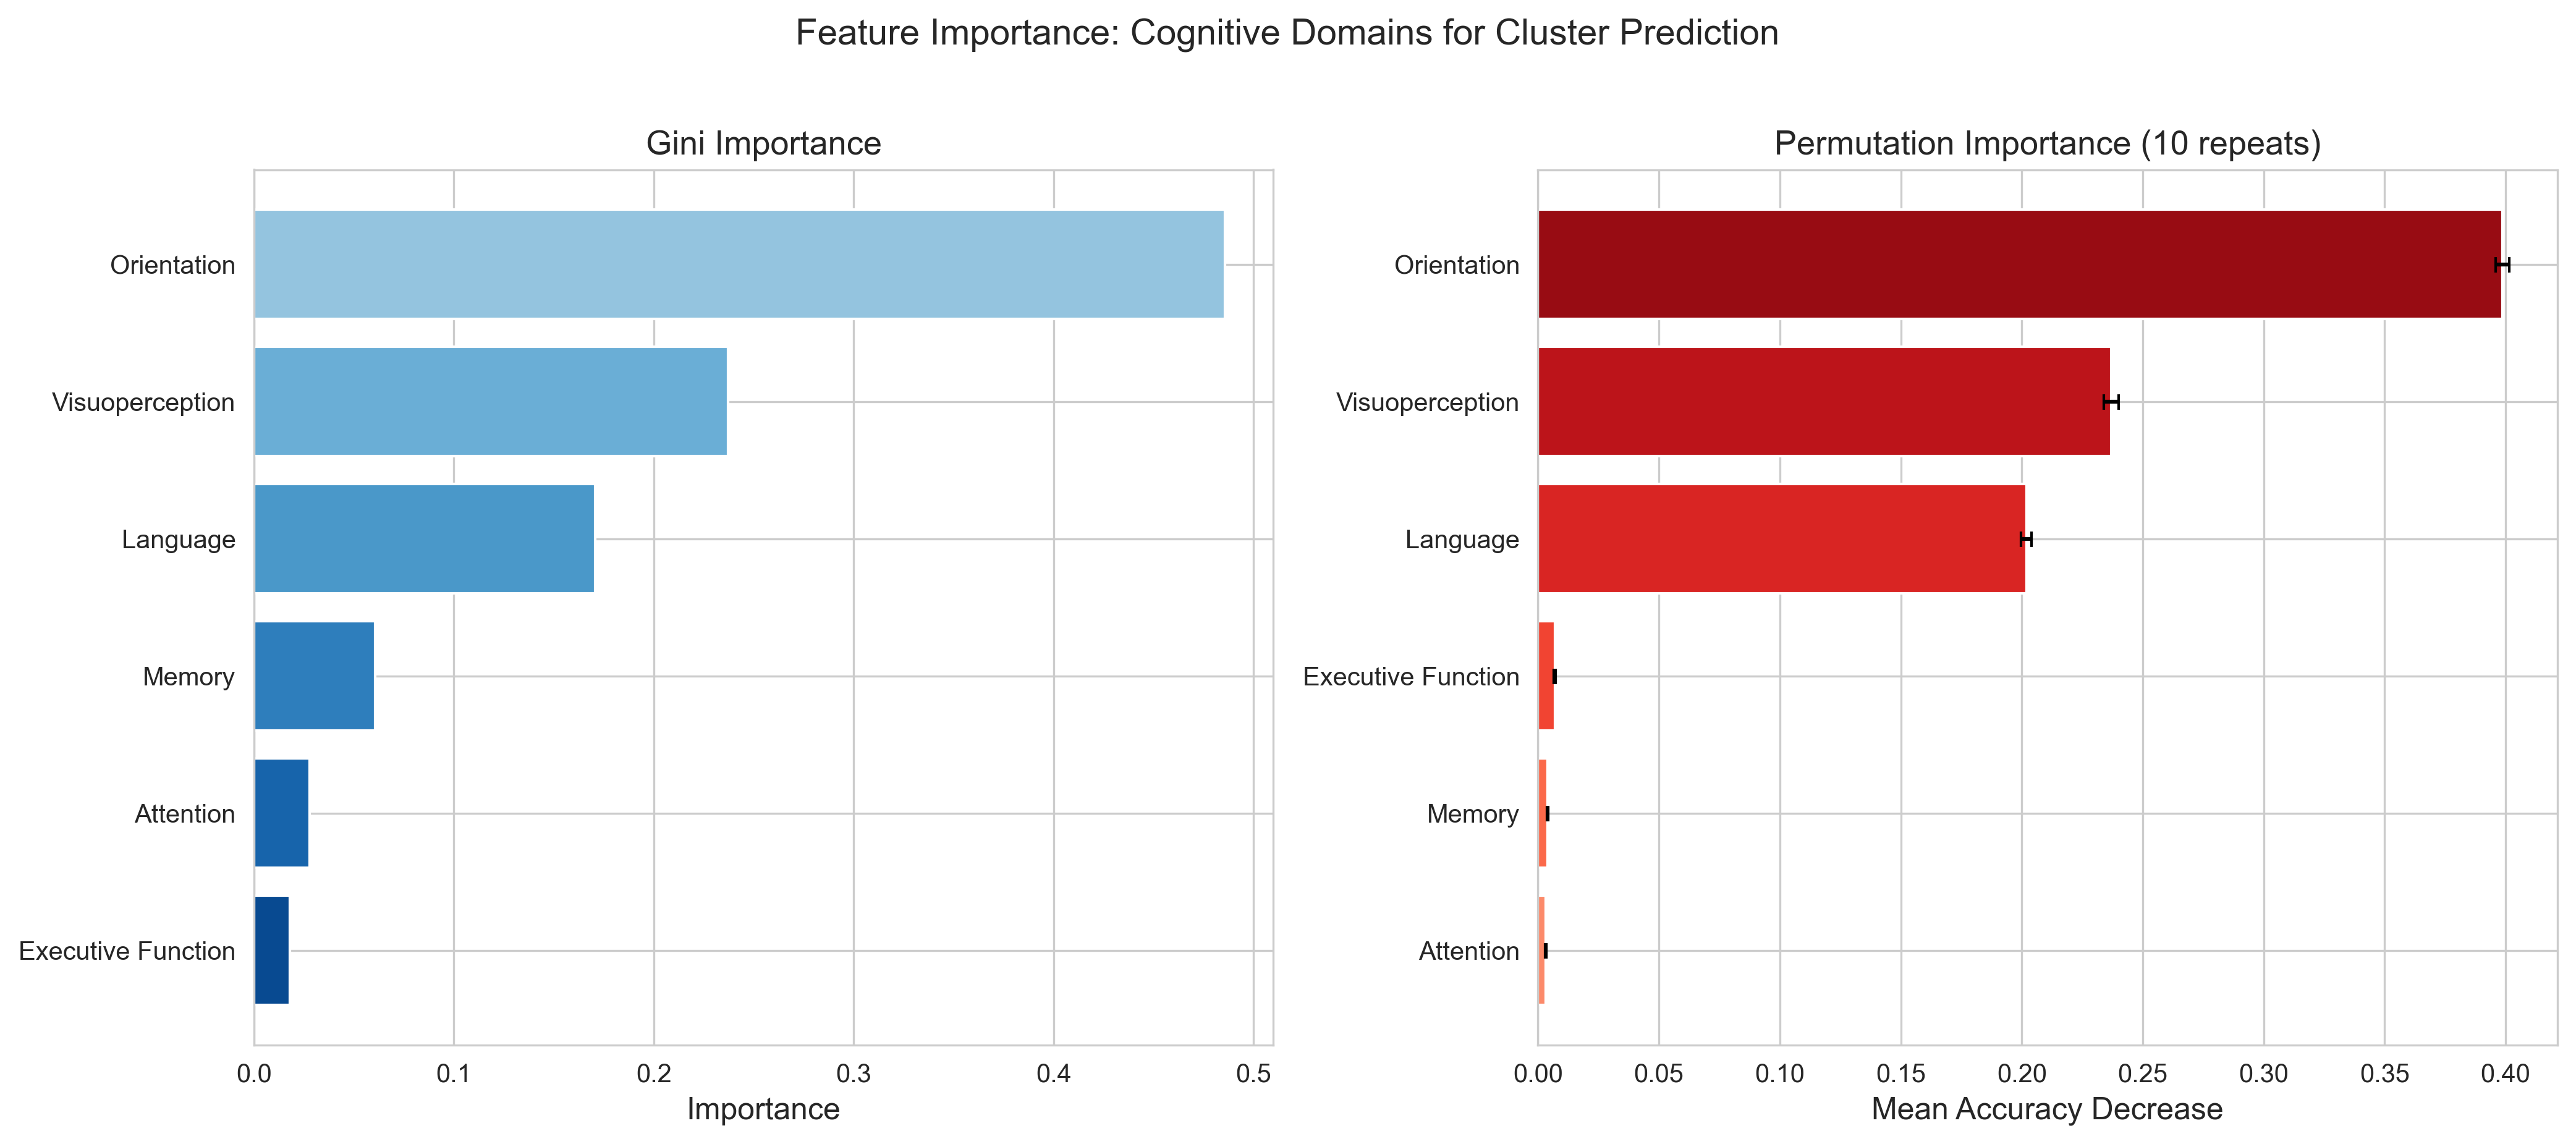
\includegraphics[width=0.9\textwidth]{Figures/feature_importance.png}
\caption[Feature importance for cluster prediction]{Random Forest surrogate trained to recover the tier labels from the domain scores. Left: Gini importance. Right: permutation importance with error bars. Because the labels derive from the same scores, this re-describes the clustering's decision boundaries rather than measuring independent importance; the ranking is also sensitive to the strong inter-domain correlation (see text) and should not be read as evidence that attention is clinically unimportant.}
\label{fig:feature_importance}
\end{figure}

%----------------------------------------------------------------------------------------
%	SECTION 10
%----------------------------------------------------------------------------------------

\section{Robustness Analyses}\label{sec:robustness}

Several robustness checks contextualise the primary hypothesis tests: a listwise-deletion baseline, subsampling stability, bootstrap confidence intervals for key estimates, Rubin-pooled uncertainty across multiple imputation draws, outcome-adjacent validation using time-since-injury, and multiple-comparison corrections for the 45 pairwise H2 tests.

\textbf{Bootstrap confidence intervals.} A non-parametric bootstrap at the patient level produced tight 95\% confidence intervals for the key estimates: 0.710 [0.704, 0.716] for the H2 mean ARI; 0.16 [0.15, 0.18] for H3 Cram\'{e}r's V; and 0.05 [0.04, 0.06] for the H4 silhouette gap (domain minus variable). These narrow intervals should be interpreted in light of the large cohort size ($n = 17{,}406$), not as evidence that all effects are large.

\textbf{H2 and multiple-comparison correction.} Testing Hypothesis~2 requires 45 pairwise ARI comparisons against the $>0.5$ threshold. I applied Holm--Bonferroni correction to control family-wise error and Benjamini--Hochberg correction for the false discovery rate, using a parametric one-sided bootstrap $p$-value for each pair. Under both corrections, 44 of the 45 pairs rejected the null at $\alpha = 0.05$. The only exception was KNN--SoftImpute (bootstrap mean ARI 0.509, 95\% CI [0.497, 0.521]), whose interval straddled the 0.5 threshold. Thus, imputation robustness holds for all method pairings except this borderline case.

\textbf{Rubin-pooled multiple imputation.} To estimate uncertainty from a single MICE run, I generated $M = 5$ independent draws, ran the full pipeline on each, and pooled the hypothesis-level metrics with Rubin's rules. The estimates remained positive and bounded: 0.154 [0.049, 0.259] for Cram\'{e}r's V (H3) and 0.050 [0.043, 0.058] for the silhouette gap (H4). The recovered cluster count varied from three to seven across draws, as expected when discretising a continuous gradient, but the H4 gap was stable. Domain-level features outperformed variable-level features in every independent draw.

\textbf{Listwise-deletion baseline.} Applying the pipeline to the 9{,}245 complete cases produced two clusters with a silhouette of 0.257. Agreement with the MICE solution for those same patients was moderate (ARI 0.625, NMI 0.519), but the solutions were not equivalent. Imputation materially affects the analysis: discarding the 46.9\% of assessments with missing values changes both the quality and number of tiers recovered.

\textbf{Subsampling stability.} Random 80\% subsamples processed with UMAP+HDBSCAN recovered the same broad severity structure, but exact labels and cluster counts varied from two to five. This is expected when a continuous gradient is converted into discrete categories and is consistent with the per-cluster Jaccard results for Hypothesis~1.

\textbf{Missingness-threshold sensitivity.} I re-ran the full process, including variable filtering, domain recomputation, MICE imputation, and UMAP+HDBSCAN, at five Tier~1 thresholds from 30\% to 70\%. As Figure~\ref{fig:sensitivity} shows, the solution remained in the two-to-three tier range with silhouettes from 0.39 to 0.52 for thresholds between 40\% and 70\%. It broke down only at the 30\% threshold, which was too restrictive and left too few variables. The 50\% threshold used in the main analysis is therefore a reasonable compromise between completeness and variable availability.

\textbf{Outcome-adjacent validation.} Functional outcome variables are unavailable, but within-patient change can be examined through time-since-injury (TSI) at assessment. TSI varies significantly by tier (Kruskal--Wallis test, $p = 4 \times 10^{-28}$): medians are 214 days for Above-Average, 188 for Near-Normal, and 172 for Global Impairment. More impaired patients are assessed slightly earlier after injury. Among the 5{,}206 patients with two or more assessments, 50.2\% ($n = 2{,}613$) remain in the same tier and 49.8\% ($n = 2{,}593$) change tier. Such mobility is more consistent with movement along a severity gradient than with fixed phenotypes. Among the 912 patients with exactly two assessments who change tier, movement toward better function is about three times more frequent than movement toward worse function (706 vs.\ 206 transitions), matching the expected clinical recovery pattern.

\begin{figure}[!ht]
\centering
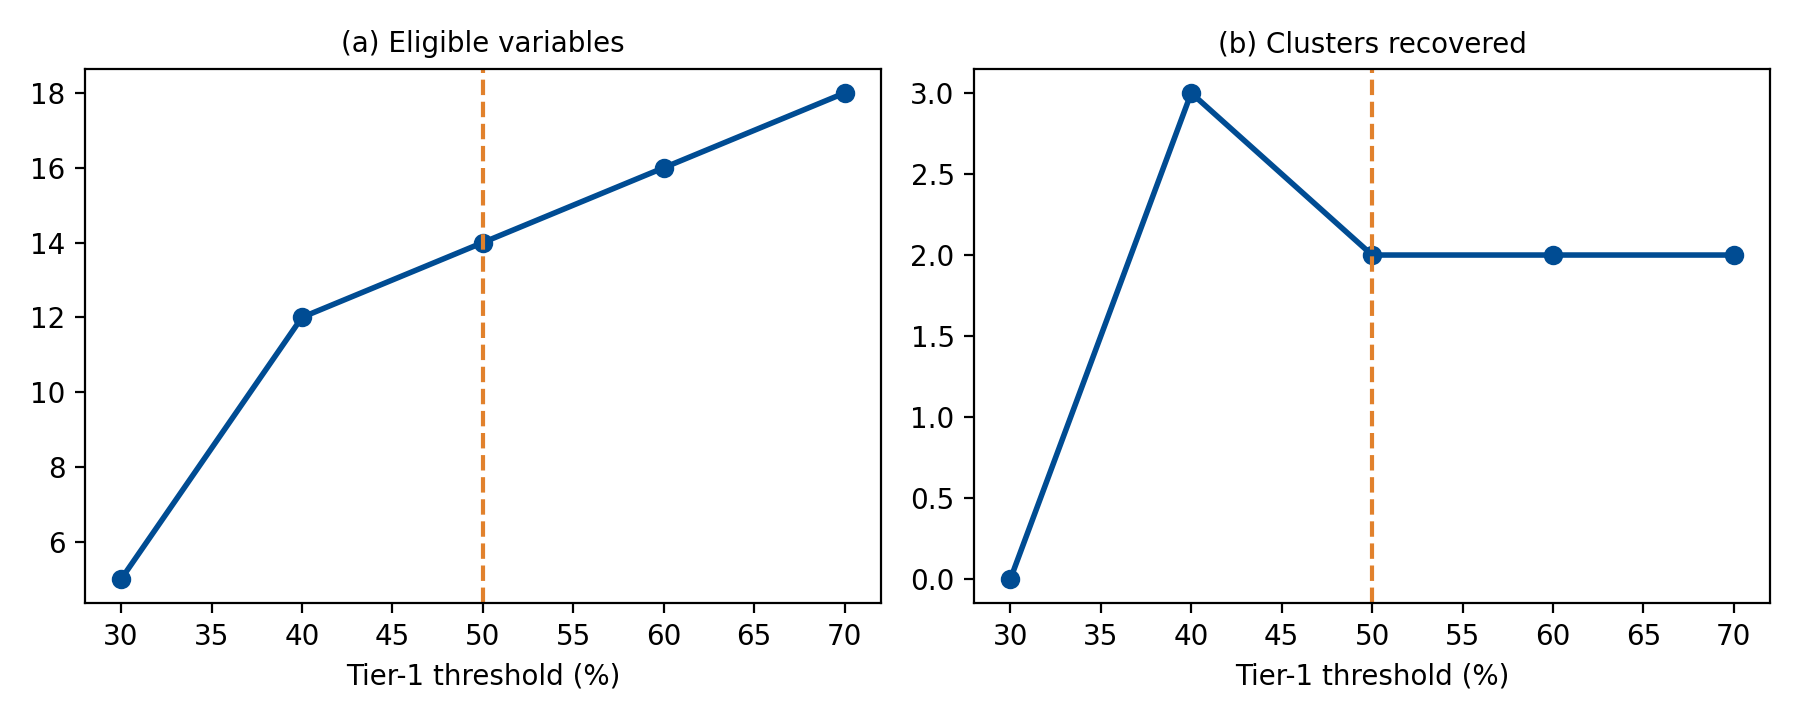
\includegraphics[width=0.8\textwidth]{Figures/sensitivity_analysis_a.png}\\[0.5em]
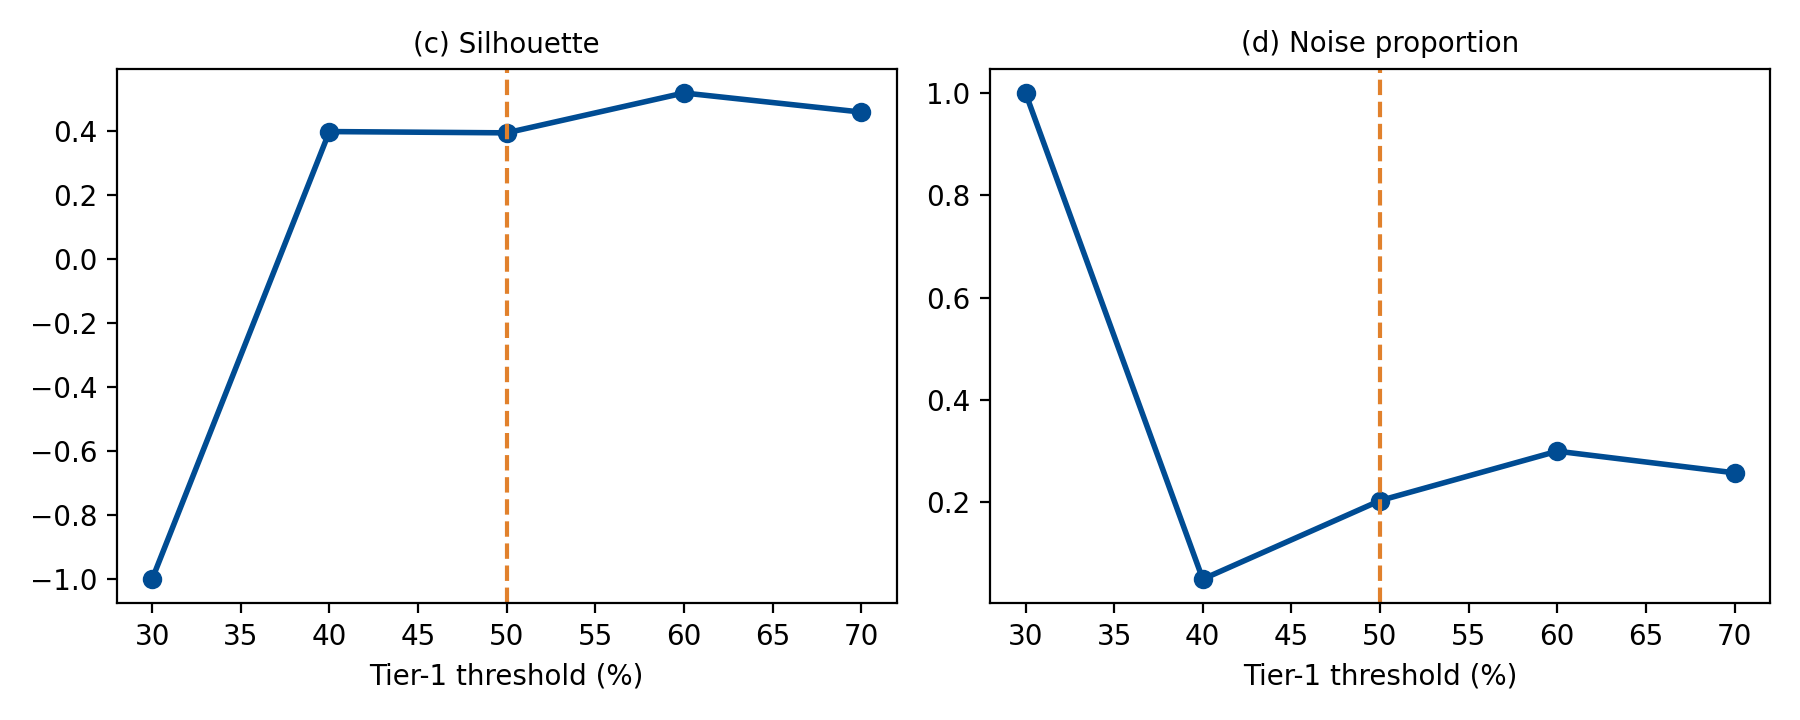
\includegraphics[width=0.8\textwidth]{Figures/sensitivity_analysis_b.png}
\caption[Sensitivity to missingness threshold]{Sensitivity to the Tier~1 missingness threshold across five values (30--70\%). Top row: (a)~number of eligible variables and (b)~number of clusters recovered. Bottom row: (c)~silhouette score and (d)~noise proportion. Dashed line marks the 50\% threshold used in the primary analysis.}
\label{fig:sensitivity}
\end{figure}

\textbf{Embedding-seed stability.} To check whether the partition depended on UMAP's stochastic initialisation, I re-ran the full embedding-and-clustering pipeline on the MICE-imputed domain scores using ten random seeds with identical hyperparameters. The label sets were highly concordant: the mean pairwise ARI across the ten runs was 0.957 (median 0.96, range 0.90--1.00), increasing to 0.965 after $k$-nearest-neighbour reassignment. The recovered structure is therefore not driven by random initialisation. Together with the deterministic PCA support for the severity axis (§\ref{sec:cluster_profiles}), this reduces concern that the result is an unstable artefact of UMAP.

\textbf{Latent-profile baseline.} As a model-based comparison, I fitted Gaussian mixture models with full covariance, corresponding to the engine of latent profile analysis, to the domain scores for $k$ from 2 to 6. The Bayesian Information Criterion fell monotonically with $k$ (from 243{,}249 at $k=2$ to 92{,}606 at $k=6$) with no local minimum, a pattern more consistent with a continuum than with well-separated latent classes. The mixture solutions agreed only moderately with the density-based tiers (ARI 0.35--0.40), and the two-component solution had the clearest silhouette (0.45). This model-based baseline therefore supports the same conclusion as the main pipeline: there is no clear discrete-class optimum, consistent with an underlying severity gradient.

\textbf{MNAR tipping-point.} To bound the possible effect of a missing-not-at-random mechanism, I re-imputed every missing value to the worst observed performance on its variable: the minimum value, or the maximum for the timed ATMTA. This is an intentionally extreme and pessimistic assumption. Under this scenario, the partition fragmented and the silhouette fell to 0.03 because forcing all missing values to a single extreme created point-mass spikes. Even so, a distinct lowest-severity tier persisted and retained 65.2\% of the assessments originally assigned to Global Impairment. The Global Impairment tier is therefore the most robust part of the solution. The extreme MNAR assumption mainly degrades the finer separation among milder tiers, and a formal delta-shifted tipping-point analysis would be a useful extension.

\textbf{Characteristics of excluded records.} Reconstructing the Tier-1 filter on the full raw cohort retained roughly 16{,}600 of the 22{,}075 records, close to the 17{,}406 used in the main analysis, and excluded about 5{,}500. The excluded records completed only 0.8 of the 14 eligible tests on average, compared with 12.5 among retained records. They therefore appear to be near-empty administrative encounters rather than partially tested, severely impaired patients. The two groups were demographically similar (age at injury 45.7 vs.\ 46.3 years, Cohen's $d = -0.04$; 63\% vs.\ 68\% male; time-since-injury 2.3 vs.\ 1.6 years, $d = 0.16$). The filter is therefore unlikely to hide a severe subgroup on measurable characteristics, although the cognitive severity of excluded records cannot be observed directly.

\clearpage

%----------------------------------------------------------------------------------------
%	SECTION 11
%----------------------------------------------------------------------------------------

\section{Cluster Clinical Naming}\label{sec:cluster_names}

A rule-based labeller was used to assign descriptive names from the domain-level $z$-score profile of each cluster. Clusters with most domains above $+0.5$ were labelled Above-Average; clusters mostly below $-0.5$ were labelled Global Impairment; and clusters near the cohort average were labelled Near-Normal. This produced the final labels Above-Average ($n = 6{,}725$), Near-Normal ($n = 6{,}328$), and Global Impairment ($n = 4{,}353$). Because the tiers differ in overall level rather than profile shape, severity labels are more accurate than phenotype names. They provide useful shorthand for clinical discussion and rehabilitation triage. The full mapping of identifiers and assessment counts is available in the interactive CogDash dashboard.
